\chapter{Implementasi dan Pengujian}
\label{chap:implementasidanpengujian}
Bab ini membahas mengenai implementasi dan pengujian konversi \textit{SharIF Judge}.
\section{Lingkungan Implementasi dan Pengujian}
Implementasi perangkat lunak \textit{SharIF Judge} dilakukan pada dua buah lingkungan. Lingkungan pertama digunakan untuk membangun perangkat lunak sedangkan lingkungan kedua digunakan untuk melakukan pengujian. Berikut merupakan spesifikasi lingkungan implementasi dan pengujian yang digunakan:

\begin{enumerate}
	\item Lingungan Pembangunan\\
	Tabel \ref{tab:devhard} menunjukan spesifikasi perangkat keras lingkungan pembangunan.
	\begin{table}[H]
 	\caption{Perangkat Keras Lingkungan Pembangunan}
	\label{tab:devhard}
    \centering
    	\begin{tabular}{|l|l|}
    	\hline
        	\textbf{Parameter} & \textbf{Nilai} \\ \hline
        	Perangkat Keras & Macbook Pro M1 \\ \hline
        	\textit{Processor} & \textit{M1 Pro} \\ \hline
        	\textit{Random Access Memory (RAM)} & 16 GB \\ \hline
        	\textit{Storage} & 512 GB \textit{SSD} \\ \hline
    	\end{tabular}
	\end{table}
	Tabel \ref{tab:devsoft} menunjukan spesifikasi perangkat lunak lingkungan pembangunan.
 	\begin{table}[H]
 	\caption{Perangkat Lunak Lingkungan Pembangunan}
	\label{tab:devsoft}
    \centering
    	\begin{tabular}{|l|l|}
    	\hline
        	\textbf{Parameter} & \textbf{Nilai} \\ \hline
        	Sistem Operasi & \textit{MACOS Sonoma Version} 14.2 \\ \hline
        	Bahasa Pemrograman & PHP, \textit{JavaScript}, \textit{CSS}, dan \textit{HTML} \\ \hline
        	\textit{Framework} & \textit{CodeIgniter} 4.2.3 \\ \hline
        	\textit{Code Editor} & \textit{Visual Studio Code} 1.84.2 (Universal) \\ \hline
        	Perangkat Lunak Pendukung & \textit{Docker Version} 4.21.1 (114176)\\ & \textit{Debian} 11-slim\\ & \textit{Composer} 2.6.5\\ & \textit{Google Chrome Version} 119.0.6045.159 (Official Build) (arm64)\\ & \textit{MariaDB} 10.5.8 \\ & \textit{phpMyAdmin} 4.8 \\ & PHP 8.1\\ \hline
    	\end{tabular}
	\end{table}
	
	\item Lingkungan Pengujian\\
	Tabel \ref{tab:staginghard} menunjukan spesifikasi perangkat keras lingkungan pengujian.
	\begin{table}[H]
 	\caption{Perangkat Keras Lingkungan Pengujian}
	\label{tab:staginghard}
    \centering
    	\begin{tabular}{|l|l|}
    	\hline
        	\textbf{Parameter} & \textbf{Nilai} \\ \hline
        	\textit{Processor} & \textit{Regular Intel 1vCPU} \\ \hline
        	\textit{Random Access Memory (RAM)} & 512 MB \\ \hline
        	\textit{Storage} & 10 GB \textit{SSD} \\ \hline
    	\end{tabular}
	\end{table}
	Tabel \ref{tab:stagingsoft} menunjukan spesifikasi perangkat lunak lingkungan pengujian.
 	\begin{table}[H]
 	\caption{Perangkat Lunak Lingkungan Pengujian}
	\label{tab:stagingsoft}
    \centering
    	\begin{tabular}{|l|l|}
    	\hline
        	\textbf{Parameter} & \textbf{Nilai} \\ \hline
        	Sistem Operasi & Ubuntu 20.04 \\ \hline
        	Perangkat Lunak Pendukung & \textit{Apache Server} 2.4.41\\ & \textit{Composer} 2.6.3\\ & \textit{MariaDB} 10.3.38 \\ & PHP 8.1.23\\ & \textit{phpMyAdmin} 4.9.5\\ \hline
    	\end{tabular}
	\end{table}
\end{enumerate}

\section{Implementasi}
Struktur aplikasi \textit{SharIF Judge} dipindahkan seperti pemetaan pada bab \ref{chap:analisis} gambar \ref{fig:dirMapping}. Pemindahan dilakukan dengan penyesuaian dan perubahan beberapa sintaks dan fungsi yang digunakan. Berikut merupakan hasil implementasi dari analisis dan perancangan perangkat lunak yang telah dibentuk:
\subsection{Instalasi \textit{CodeIgniter 4}}
\textit{CodeIgniter 4} diinstalasi menggunakan \textit{composer}. \textit{Composer} merupakan sebuah \textit{dependency manager} untuk PHP yang memungkinkan pengguna untuk melakukan instalasi seluruh kebutuhan untuk menjalankan program berbasis PHP. Instalasi akan dilakukan menggunakan sintaks sebagai berikut:

\begin{center}
\verb|composer create-project codeigniter4/appstarter SharIF-JudgeCI4|
\end{center}

Sintaks diatas akan mengunduh dan melakukan instalasi \textit{template} projek \textit{CodeIgniter 4}. Template berisikan \textit{skeleton} dari projek \textit{CodeIgniter 4} yang berisikan data untuk melakukan \textit{development} sebuah aplikasi.

\subsection{app/Config}
\textit{File} \textit{config} pada \textit{CodeIgniter 3} dipindahkan sesuai dengan pemetaan pada gambar \ref{fig:dirMapping}. Direktori berisikan data-data pada \texttt{application/Config}. Beberapa data pada direktori ini dipindahkan menuju \textit{file} yang terdapat pada \textit{CodeIgniter 4}. Terdapat juga penambahan \textit{file} \texttt{Secrets.php} yang dibentuk secara manual. Berikut merupakan rincian isi direktori yang dipindahkan:
\subsubsection{\texttt{app/Config/App.php}}
\textit{File} ini tidak digunakan sehingga dibiarkan berisi sintaks \textit{default} dan seluruh data akan dipindahkan menuju \textit{file} \texttt{.env}. Kode \ref{kode:envfileapp} menunjukan isi dari \textit{file} \texttt{.env} yang dipindahkan dari direktori \texttt{application/config.php}:

\begin{lstlisting}[caption= Kode \texttt{application/config/config.php} yang dipindahkan menuju \texttt{.env}, label=kode:envfileapp]
	app.baseURL = 'http://sharif.localhost/'
\end{lstlisting}

Kode \ref{kode:envfileapp} akan menentukan URL dasar dari aplikasi menjadi \texttt{http://sharif.localhost/}. URL dibentuk spesifik berupa \texttt{http://sharif.localhost/} karena dijalankan pada server lokal sehingga tidak bertabrakan dengan server lokal lainnya. URL juga diganti karena tidak dapat diimplementasikan pada \textit{CodeIgniter 4} sehingga URL ditentukan manual sesuai dengan \textit{domain} yang dibentuk.

\subsubsection{\texttt{app/Config/Autoload.php}}
\textit{File} ini tidak digunakan dan dibiarkan menggunakan konfigurasi \textit{default} karena terdapat perubahan cara kerja kelas ini. Fitur ini pada \textit{CodeIgniter 4} tidak dapat melakukan inisiasi otomatis terhadap \textit{model, controller}, dan \textit{library} saat aplikasi dijalankan. Namun kelas ini hanya akan mencari lokasi \textit{file} sesuai dengan konfigurasinya saat kelas tersebut pertama kali diinisiasi. Kelas \textit{helpers} yang diinisiasikan dipindahkan menuju \texttt{BaseController} sedangkan kelas \textit{model} dan \textit{libraries} akan dipanggil menggunakan \textit{PSR-4} pada \textit{file-file} yang membutuhkan kelas tersebut.

\subsubsection{\texttt{app/Config/Cache.php}}
\textit{File} tidak berubah dan akan tetap menggunakan konfigurasi \textit{default} karena tidak terdapat perubahan pada \textit{SharIF Judge} versi \textit{CodeIgniter 3}.

\subsubsection{\texttt{app/Config/Constants.php}}
\textit{File} ini berisikan seluruh data yang dipindahkan dari \texttt{application/config/constants.php}. Kode \ref{kode:constantbab4} menunjukan data yang dipindahkan menuju \texttt{Constant.php}.

\begin{lstlisting}[language=PHP, caption=Pemindahan kode pada \textit{Constant}, label=kode:constantbab4]
define('SHJ_VERSION','1.4');

/*Code editor related constants*/
define('EDITOR_FILE_NAME', "editor");
define('EDITOR_FILE_EXT', "txt");
define('EDITOR_IN_NAME', "exec_in");
define('EDITOR_OUT_NAME', "exec_out");
define('EDITOR_SUBMIT_ID', 0);
\end{lstlisting}

Kode \ref{kode:constantbab4} menunjukan pemindahan data dari \textit{file} \texttt{application/config/constants.php} menuju \texttt{Constant.php}. Sintaks \texttt{SHJ\_VERSION} akan digunakan pada tampilan \texttt{sidebar} sedangkan sintaks \texttt{EDITOR} digunakan pada fungsi \textit{submit}. Sintaks yang telah dipindahkan akan bersifat \textit{global} sehingga dapat diakses oleh seluruh \textit{file} pada \textit{CodeIgniter 4}.

\subsubsection{\texttt{app/Config/Cookie.php}}
\textit{File} ini tidak terdapat perubahan dan tetap menggunakan konfigurasi \textit{default} karena tidak terdapat perubahan pada \textit{SharIF Judge} versi \textit{CodeIgniter 3}.

\subsubsection{\texttt{app/Config/Database.php}}
\textit{File} ini dibiarkan menggunakan konfigurasi \textit{default} karena akan dipindahkan menuju \textit{file} \texttt{.env}. Kode \ref{kode:databaseenvbab4} menunjukan pemindahan menuju \textit{file} \texttt{.env} yang dipindahkan dari \textit{file} \texttt{application/config.php}.

\begin{lstlisting}[caption=Pemindahan \texttt{app/config/database.php} menuju \texttt{.env}, label=kode:databaseenvbab4]
database.default.hostname = db
database.default.database = sharif
database.default.username = root
database.default.password = 
database.default.DBDriver = MySQLi
database.default.DBPrefix = shj_
\end{lstlisting}

Kode \ref{kode:databaseenvbab4} menunjukan pemindahan kode dari \texttt{database.php} menuju \texttt{.env}. Kode akan berisikan \textit{hostname} yang digunakan, nama \textit{database} yang digunakan, \textit{username} dari \textit{database}, \textit{password}, \textit{DBDriver}, dan \textit{DBPrefix} yang digunakan.

\subsubsection{\texttt{app/Config/Email.php}}
\textit{File} ini tidak digunakan dan dibiarkan menggunakan konfigurasi \textit{default} karena konfigurasi \textit{email} pada aplikasi \textit{SharIF Judge} diletakan pada \textit{file} \texttt{Secrets.php}.

\textit{File} ini berisikan seluruh data yang dipindahkan dari \texttt{application/config/secrets.php}. Kode \ref{kode:emailconfigbab4} menunjukan pemindahan konfigurasi \textit{email}.

\begin{lstlisting}[language=PHP, caption=Pemindahan \texttt{app/config/secrets.php} menuju \texttt{Email.php}, label=kode:emailconfigbab4]
    public string $protocol = 'smtp';
    public string $SMTPHost = 'ssl://smtp.mailgun.org';
    public string $mailType = 'html';
\end{lstlisting}

Kode \ref{kode:emailconfigbab4} menunjukan pemindahan konfigurasi \textit{email} yang terdapat pada \texttt{secrets.php}. Kode akan berisikan \textit{protocol} yang digunakan untuk mengirim \textit{email}, \textit{host} yang akan digunakan, dan tipe \textit{email} yang dikirimkan. Seluruh data akan disimpan menuju variabel pada \textit{CodeIgniter 4} dan terdapat perubahan nama variabel menjadi \textit{camelCase}.

\subsubsection{\texttt{app/Config/Encryption.php}}
\textit{File} ini berisikan seluruh data yang dipindahkan dari \texttt{application/config/config.php}. Kode \ref{kode:encryptionbab4} menunjukan pemindahan konfigurasi enkripsi yang akan digunakan.

\begin{lstlisting}[language=PHP, caption=Pemindahan \texttt{app/config/config.php} menuju \texttt{Encryption.php}, label=kode:encryptionbab4]
    public string $key = 'bj42CAiqTwLHUhz3pOvfRM0EJFeQD9uG';
\end{lstlisting}

Kode \ref{kode:encryptionbab4} menunjukan pemindahan \textit{key} dari enkripsi yang akan digunakan. Data akan disimpan menuju variabel pada \textit{CodeIgniter 4}.

\subsubsection{\texttt{app/Config/Filters.php}}
\label{subsubsec:filters}
\textit{File} ini berisikan seluruh nama \textit{filters} yang telah dibentuk. Kode \ref{kode:filtersnamebab4} menunjukan pembangunan nama \textit{filters} sesuai dengan kelas yang sudah dibentuk.

\begin{lstlisting}[language=PHP, caption=Penambahan nama \textit{filters} untuk didefinisikan menuju \textit{routes}, label=kode:filtersnamebab4]
	public array $aliases = [
        'csrf'          => CSRF::class,
        'toolbar'       => DebugToolbar::class,
        'honeypot'      => Honeypot::class,
        'invalidchars'  => InvalidChars::class,
        'secureheaders' => SecureHeaders::class,
        'check-installandlogin' => CheckInstallAndLogin::class,
        'check-login' => CheckLogin::class,
        'check-loginandlevelAdmin' => CheckLoginandLevelAdmin::class,
        'check-loginandlevelHead' => CheckLoginandLevelHead::class,
        'check-loginandcli' => CheckLoginandCLI::class,
        'check-loginandisajax' => CheckLoginandisAjax::class,
        'check-iscli' => CheckCLI::class,
     ]
\end{lstlisting}

Kode \ref{kode:filtersnamebab4} menunjukan penambahan nama \textit{filters} untuk dipanggil menuju \textit{routes}. Penamaan ini akan ditambahkan pada \textit{array} \verb|$aliases| dengan nama lain \textit{filters} dan nama kelasnya.
\subsubsection{\texttt{app/Config/Routes.php}}
\textit{File} ini berisikan seluruh pemindahan dan penambahan manual dari \textit{routes} pada \textit{SharIF Judge}. Kode \ref{kode:routesbab4} menunjukan pembangunan \textit{routes} aplikasi secara manual.
\begin{lstlisting}[language=PHP, caption=Penambahan \textit{routes} yang digunakan pada aplikasi \textit{SharIF Judge}, label=kode:routesbab4]
	$routes->setDefaultNamespace('App\Controllers');
$routes->setDefaultController('Dashboard');
$routes->setDefaultMethod('index');
$routes->setTranslateURIDashes(false);
$routes->set404Override();
$routes->setAutoRoute(false);
// The Auto Routing (Legacy) is very dangerous. It is easy to create vulnerable apps
// where controller filters or CSRF protection are bypassed.
// If you don't want to define all routes, please use the Auto Routing (Improved).
// Set `$autoRoutesImproved` to true in `app/Config/Feature.php` and set the following to true.
// $routes->setAutoRoute(false);

/*
 * --------------------------------------------------------------------
 * Route Definitions
 * --------------------------------------------------------------------
 */

// We get a performance increase by specifying the defaul
// route since we don't have to scan directories.
$routes->get('/', 'Dashboard::index',['filter' => 'check-installandlogin:dual,noreturn']);
$routes->get('/dashboard', 'Dashboard::index',['filter' => 'check-installandlogin:dual,noreturn']);
$routes->post('/dashboard/widget_positions', 'Dashboard::widget_positions');
// Authentication
$routes->add('/install','Install::index');
$routes->add('/login','Login::index');
$routes->post('login/register','Login::register');
$routes->get('login/lost','Login::lost');
$routes->post('login/lost','Login::lost');
$routes->get('/reset/(:any)', 'Login::reset/$1');
$routes->post('login/reset/(:any)', 'Login::reset/$1');
$routes->get('/register','Login::register');
$routes->post('/register','Login::register');
$routes->get('/settings','Settings::index',['filter' => 'check-loginandlevelAdmin:dual,noreturn']);
$routes->post('/settings','Settings::index',['filter' => 'check-loginandlevelAdmin:dual,noreturn']);
$routes->add('/profile/(:num)','Profile::index/$1',['filter' => 'check-login:dual,noreturn']);
$routes->get('/logout','Login::logout');
$routes->add('/settings/update', 'Settings::update');
// Users
$routes->get('/profile', 'Profile::index');
$routes->get('/users', 'Users::index',['filter' => 'check-loginandlevelAdmin:dual,noreturn']);
$routes->get('/users/add', 'Users::add',['filter' => 'check-loginandlevelAdmin:dual,noreturn']);
$routes->post('/users/add', 'Users::add',['filter' => 'check-loginandlevelAdmin:dual,noreturn']);
$routes->post('/users/delete_submissions', 'Users::delete_submissions',['filter' => 'check-loginandlevelAdmin:dual,noreturn']);
$routes->get('users/list_excel', 'Users::list_excel',['filter' => 'check-loginandlevelAdmin:dual,noreturn']);
// Notifications and scoreboard
$routes->get('/notifications', 'Notifications::index',['filter' => 'check-login:dual,noreturn']);
$routes->get('/notifications/add', 'Notifications::add',['filter' => 'check-login:dual,noreturn']);
$routes->post('/notifications/add', 'Notifications::add',['filter' => 'check-login:dual,noreturn']);
$routes->add('/notifications/edit/(:num)', 'Notifications::edit/$1',['filter' => 'check-login:dual,noreturn']);
$routes->post('/notifications/delete', 'Notifications::delete',['filter' => 'check-login:dual,noreturn']);
$routes->post('/notifications/check', 'Notifications::check',['filter' => 'check-login:dual,noreturn']);
$routes->get('/scoreboard','Scoreboard::index',['filter' => 'check-loginandcli:dual,noreturn']);
$routes->add('/server_time','Server_time::index',['filter' => 'check-loginandisajax:dual,noreturn']);
// Logs, hof, moss, rejudge, queue
$routes->get('logs', 'Logs::index',['filter' => 'check-login:dual,noreturn']);
$routes->get('halloffame', 'Halloffame::index',['filter' => 'check-login:dual,noreturn']);
$routes->get('moss/(:num)','Moss::index/$1',['filter' => 'check-loginandlevelHead:dual,noreturn']);
$routes->post('moss/(:num)','Moss::index/$1',['filter' => 'check-loginandlevelHead:dual,noreturn']);
$routes->get('moss/update/(:num)','Moss::update/$1',['filter' => 'check-loginandlevelHead:dual,noreturn']);
$routes->post('moss/update/(:num)','Moss::update/$1',['filter' => 'check-loginandlevelHead:dual,noreturn']);
$routes->get('queue','Queue::index',['filter' => 'check-loginandlevelHead:dual,noreturn']);
$routes->post('queue','Queue::index',['filter' => 'check-loginandlevelHead:dual,noreturn']);
$routes->post('queue/resume','Queue::resume',['filter' => 'check-loginandlevelHead:dual,noreturn']);
$routes->post('queue/pause','Queue::pause',['filter' => 'check-loginandlevelHead:dual,noreturn']);
$routes->post('queue/empty_queue','Queue::empty_queue',['filter' => 'check-loginandlevelHead:dual,noreturn']);
$routes->cli('queueprocess/run', 'Queueprocess::run');
$routes->get('rejudge', 'Rejudge::index',['filter' => 'check-loginandlevelHead:dual,noreturn']);
$routes->post('rejudge', 'Rejudge::index',['filter' => 'check-loginandlevelHead:dual,noreturn']);
$routes->get('rejudge/(:num)', 'Rejudge::index/$1',['filter' => 'check-loginandlevelHead:dual,noreturn']);
$routes->post('rejudge/rejudge_single','Rejudge::rejudge_single',['filter' => 'check-loginandlevelHead:dual,noreturn']);
//Assignments
$routes->get('/assignments','Assignments::index',['filter' => 'check-login:dual,noreturn']);
$routes->get('/assignments/add','Assignments::add',['filter' => 'check-login:dual,noreturn']);
$routes->post('/assignments/add','Assignments::add',['filter' => 'check-login:dual,noreturn']);
$routes->post('/assignments/select','Assignments::select',['filter' => 'check-login:dual,noreturn']);
$routes->get('/assignments/edit/(:num)','Assignments::edit/$1',['filter' => 'check-login:dual,noreturn']);
$routes->post('/assignments/edit/(:num)','Assignments::edit/$1',['filter' => 'check-login:dual,noreturn']);
$routes->get('/assignments/delete/(:num)','Assignments::delete/$1',['filter' => 'check-login:dual,noreturn']);
$routes->post('/assignments/delete/(:num)','Assignments::delete/$1',['filter' => 'check-login:dual,noreturn']);
$routes->get('/assignments/pdf/(:num)/(:any)/(:any)','Assignments::pdf/$1/$2/$3',['filter' => 'check-login:dual,noreturn']);
$routes->get('/assignments/pdf/(:num)','Assignments::pdf/$1',['filter' => 'check-login:dual,noreturn']);
$routes->post('/assignments/pdfCheck/(:num)', 'Assignments::pdfCheck/$1');
$routes->get('/assignments/pdfCheck/(:num)', 'Assignments::pdfCheck/$1');
$routes->get('assignments/downloadtestsdesc/(:num)', 'Assignments::downloadtestsdesc/$1');
$routes->get('assignments/download_submissions/(:any)/(:num)', 'Assignments::download_submissions/$1/$2');
// Submit and submissions
$routes->get('submit','Submit::index',['filter' => 'check-login:dual,noreturn']);
$routes->post('submit','Submit::index',['filter' => 'check-login:dual,noreturn']);
$routes->get('submit/load/(:num)','Submit::load/$1',['filter' => 'check-login:dual,noreturn']);
$routes->post('submit/save/(:any)','Submit::save/$1');
$routes->post('submit/save','Submit::save');
$routes->get('submit/get_output/(:num)','Submit::get_output/$1');
$routes->get('submissions/all/user/(:any)', 'Submissions::all');
$routes->get('submissions/final','Submissions::the_final',['filter' => 'check-login:dual,noreturn']);
$routes->get('submissions/final/(:any)','Submissions::the_final/$1',['filter' => 'check-login:dual,noreturn']);
$routes->post('/submissions/view_code', 'Submissions::view_code');
$routes->post('/submissions/select', 'Submissions::select');
$routes->get('/submissions/all_excel', 'Submissions::all_excel');
$routes->get('/submissions/final_excel', 'Submissions::final_excel');
$routes->get('submissions/download_file/(:any)/(:num)/(:num)/(:num)','Submissions::download_file/$1/$2/$3/$4');
$routes->get('submissions/all','Submissions::all');
// Problems
$routes->get('/problems', 'Problems::index',['filter' => 'check-login:dual,noreturn']);
$routes->get('/problems/(:num)','Problems::index/$1');
$routes->get('/problems/(:num)/(:num)','Problems::index/$1/$2');
$routes->get('/problems/edit/(:any)/(:num)/(:num)', 'Problems::edit/$1/$2/$3');
$routes->post('/problems/edit/(:any)/(:num)/(:num)', 'Problems::edit/$1/$2/$3');
\end{lstlisting}
Kode \ref{kode:routesbab4} menunjukan seluruh \textit{routes} yang didefinisikan secara explisit sesuai dengan kegunaannya. Terdapat juga penambahan \textit{filters} untuk melakukan pengecekan sebelum \textit{controller} diinisiasikan. Pembangunan \textit{routes} secara manual dilakukan karena alasan keamanan dan juga konfigurasi \textit{filters} yang berbeda untuk setiap \textit{controller}.

\subsubsection{\texttt{app/Config/Secrets.example.php}}
\textit{File} ini merupakan \textit{file} yang ditambahkan diluar dari struktur standart dari aplikasi \textit{CodeIgniter 4}. \textit{File} ini berisikan seluruh kebutuhan konfigurasi yang tidak terdapat pada \textit{config} lainnya. Kode \ref{kode:secrets} menunjukan pemindahan \textit{file} \texttt{secrets.example.php} menuju \texttt{app/Config/Secrets.example.php}.
\begin{lstlisting}[language=PHP, caption=Penambahan \textit{file} \texttt{Secrets.example.php}, label=kode:secrets]
namespace Config;

use CodeIgniter\Config\BaseConfig;
class Secrets extends BaseConfig
{ 
	public $shj_authenticate = 'radius';

public $shj_radius = [
    "server" => "localhost",
    "secret" => "i-have-no-secret"
];

// LDAP Settings reffers to
// @link https://adldap2.github.io/Adldap2/#/setup?id=options
public $shj_ldap = [
    "hosts" => ["dc3.ftis.unpar"],
    "base_dn" => "DC=FTIS,DC=UNPAR",
    "username"=> "",
    "password"=> "",
    "account_suffix"   => "@ftis.unpar"
];

public $shj_mail = [
    'protocol' => 'smtp',
    'SMTPHost' => 'ssl://smtp.mailgun.org',
    'SMTPPort' => 465,
    'SMTPUser' => '',
    'SMTPPass' => '',
    'mailType'  => 'html',
    'charset'   => 'utf-8'
];
}
\end{lstlisting}

Kode \ref{kode:secrets} menunjukan pemindahan kode menuju \texttt{app/Config}. Terdapat penghapusan sintaks \texttt{defined('BASEPATH') OR exit('No direct script access allowed');} pada baris pertama kalimat. Sintaks yang telah dihapus akan digantikan oleh sintaks \textit{class} seperti pada baris pertama dan nama kelas akan \textit{extend} \texttt{BaseConfig}. Terdapat juga penambahan sintaks \textit{namespace} dan \textit{use}. \textit{File} ini akan digunakan dan dipanggil pada \textit{controller} untuk melakukan autentikasi dan konfigurasi \textit{email} pengguna.

\subsubsection{\texttt{app/Config/Security.php}}
\textit{File} ini berisikan seluruh konfigurasi yang dipindahkan dari \texttt{application/config/config.php}. Kode \ref{kode:security} menunjukan pemindahan data token \textit{csrf} dan \textit{cookie} menuju \texttt{Security.php}.
\begin{lstlisting}[language=PHP, caption=Pemindahan \textit{file} \textit{config} menuju \texttt{Security.php}, label=kode:security]
public string $tokenName = 'shj_csrf_token';
public string $cookieName = 'shjcsrftoken';
\end{lstlisting}

Kode \ref{kode:security} menunjukan pemindahan sintaks menuju \texttt{Security.php}. Sintaks pada baris pertama merupakan nama \textit{token} yang akan digunakan sedangkan sintaks kedua merupakan nama \textit{cookie} yang akan digunakan. Sintaks pada \textit{CodeIgniter 4} tidak akan menggunakan \textit{array} namun akan disimpan menuju variabel. Sintaks lainnya tidak akan diubah karena akan menggunakan konfigurasi \textit{default} dari \textit{CodeIgniter 4}.

\subsubsection{\texttt{app/Config/Session.php}}
\textit{File} ini berisikan seluruh konfigurasi yang dipindahkan dari \texttt{application/config/config.php}. Kode \ref{kode:session} menunjukan pemindahan data konfigurasi \textit{session} menuju \texttt{Session.php}.
\begin{lstlisting}[language=PHP, caption=Pemindahan \textit{file} \textit{config} menuju \texttt{Session.php}, label=kode:session]
public string $driver = 'CodeIgniter\Session\Handlers\DatabaseHandler';
public string $cookieName = 'shjsession';
\end{lstlisting}

Data yang dipindahkan berupa \texttt{cookieName} yang selanjutnya disimpan menuju sebuah variabel. Selanjutnya terdapat perubahan \textit{driver} dimana akan menggunakan \textit{database handler} yang menyimpan data menuju \textit{database}.

\subsubsection{\texttt{app/Config/Validation.php}}
\label{subsubsec:validationbab4}
\textit{File} ini berisikan aturan yang dibentuk secara manual oleh pengguna untuk melakukan validasi sebelum \textit{request} diproses oleh aplikasi. Kode \ref{kode:validationrulesmanualbab4} menunjukan aturan validasi data yang dibentuk secara manual oleh pengguna.

\begin{lstlisting}[language=PHP, caption=Perancangan aturan yang dibentuk secara manual pada \textit{file} \texttt{Validation.php}, label=kode:validationrulesmanualbab4]
class MyRules
{   
    public function password_check($str): bool
    {
        if (strlen($str) == 0 OR (strlen($str) >= 6 && strlen($str) <= 200))
			return TRUE;
		return FALSE;
    }

    public function password_again_check($str) :bool
    {
        $request = \Config\Services::request();
        if ($request->getPost('password') !== $request->getPost('password_again'))
			return FALSE;
		return TRUE;
    }

    public function role_check($role) 
    {
        $user = new User();
        if ($user->level <= 2)
			return ($role == '');

		// Admins can change everybody's user role:
		$roles = array('admin', 'head_instructor', 'instructor', 'student');
		return in_array($role, $roles);
    }

    /**
	 * Checks whether a user with this email exists
	 */
	public function email_check($email,$edit_username):bool
	{
		$edit_username = explode(',', $edit_username);
        $user_model = new UserModel();
		if ($user_model->have_email($email, $edit_username))
			return FALSE;
		return TRUE;
	}

    /**
	 * checks whether the entered registration code is correct or not
	 *
	 */
	public function _registration_code($code){
        $settings_model = new SettingsModel();
		$rc = $settings_model->get_setting('registration_code');
		if ($rc == '0')
			return TRUE;
		if ($rc == $code)
			return TRUE;
		return FALSE;
	}

    /**
	 * Required
	 *
	 * @param	string
	 * @return	bool
	 */
	public function required($str)
	{
		return is_array($str) ? (bool) count($str) : ($str !== '');
	}


	// -------------------------------------------------------------------------


	/**
	 * Is Lowercase
	 *
	 * @param $str
	 * @return bool
	 */
	public function lowercase($str)
	{
		return (strtolower($str) === $str);
	}

    	// ------------------------------------------------------------------------


	public function _check_language($str)
	{
		if ($str=='0')
			return FALSE;
		if (in_array( strtolower($str),array('c', 'c++', 'python 2', 'python 3', 'java', 'zip', 'pdf', 'txt')))
			return TRUE;
		return FALSE;
	}


	// ------------------------------------------------------------------------
	// Used in Submissions.php

	public function _check_type($type)
	{
		return ($type === 'code' || $type === 'result' || $type === 'log');
	}
}
\end{lstlisting}

Kode \ref{kode:validationrulesmanualbab4} menunjukan pembangunan aturan secara manual yang dipindahkan dari \textit{controller} \texttt{Login.php}, \texttt{Profile.php}, \texttt{Submissions.php}, dan \texttt{Submit.php}. Aturan yang dibentuk secara manual dapat digunakan seperti aturan lainnya yang tersedia pada \textit{CodeIgniter 4}. Aturan yang dibentuk terdapat beberapa penambahan seperi pemanggilan \textit{library}, \textit{model}, dan penambahan sintaks untuk memecah \textit{array}.

\subsection{\textit{Controllers}}
\textit{Controller} terdapat perubahan pada bagian fungsi \texttt{\_\_construct()} dimana sekarang tidak dapat mengembalikan sesuatu. Oleh karena itu, akan dibentuk beberapa \textit{filters} \ref{subsubsec:filters} untuk melakukan pengecekan terhadap fungsi yang sebelumnya terdapat pada \texttt{\_\_construct()}.
	\subsubsection{app/Controllers} 
	Direktori ini berisikan seluruh \textit{controller} yang dipindahkan dari \texttt{application/controllers}. Berikut merupakan isi pada direktori ini:
	\begin{itemize}
		\item \texttt{Assignments.php}
		\item \texttt{BaseController.php}
		\item \texttt{Dashboard.php}
		\item \texttt{Halloffame.php}
		\item \texttt{Install.php}
		\item \texttt{Login.php}
		\item \texttt{Logs.php}
		\item \texttt{Moss.php}
		\item \texttt{Notifications.php}
		\item \texttt{Problems.php}
		\item \texttt{Profile.php}
		\item \texttt{Queue.php}
		\item \texttt{Queueprocess.php}
		\item \texttt{Rejudge.php}
		\item \texttt{Scoreboard.php}
		\item \texttt{Server\_time.php}
		\item \texttt{Settings.php}
		\item \texttt{Submissions.php}
		\item \texttt{Submit.php}
		\item \texttt{Users.php}
	\end{itemize}

\textit{Controllers} terdapat perubahan dan penambahan baik dalam kelas yang dilakukan \textit{extends} maupun dalam pemanggilan kelas lain seperti \textit{model} dan \textit{helpers}. Beberapa \textit{helpers} yang dipanggil melalui \textit{autoload} dipindahkan menuju \textit{BaseController}. Kode \ref{kode:controllerBab4} menunjukan perubahan yang terdapat pada \textit{controller} \texttt{Logs.php}.

\begin{lstlisting}[language=PHP, caption=Perubahan kode \textit{controller} \texttt{Logs.php} pada \textit{CodeIgniter 4}, label=kode:controllerBab4]
namespace App\Controllers;

use App\Controllers\BaseController;
use App\Models\AssignmentModel;
use App\Models\LogsModel;
use App\Models\User;

class Logs extends BaseController
{
	protected $session;
	protected $user;
	protected $logs_model;
	protected $assignment_model;

	public function __construct()
	{
		$this->session = session();
		$this->logs_model = new LogsModel();
		$this->assignment_model = new AssignmentModel();
		$this->user = new User();
		if ( $this->user->level <= 2) // permission denied
			throw \CodeIgniter\Exceptions\PageNotFoundException::forPageNotFound();
	}
	
	public function index()
	{

		$data = array(
			'logs' => $this->logs_model->get_all_logs(),
			'selected' => 'logs',
			'user' => $this->user,
			'all_assignments' => $this->assignment_model->all_assignments(),
			'finish_time' => $this->user->selected_assignment['finish_time'],
			'extra_time' => $this->user->selected_assignment['extra_time'],
		);

		return view('pages/admin/logs', $data);
	}
}
\end{lstlisting}

Kode \ref{kode:controllerBab4} terdapat perubahan dimana sekarang akan \textit{extends} \textit{BaseController}. Terdapat juga penghapusan sintaks \texttt{defined('BASEPATH') OR exit('No direct script access allowed');}. Terdapat penambahan sintaks \textit{namespace} dan juga beberapa sintaks untuk memanggil \textit{models}. \textit{Controller} juga memiliki perubahan dalam mengembalikan \textit{view} dimana sekarang menggunakan sintaks \texttt{return view}. Selain itu terdapat penambahan pada \texttt{BaseController.php} untuk melakukan inisiasi terhadap \textit{helpers} dan juga beberapa \textit{library} yang akan digunakan. Kode \ref{kode:basecontrollerhelpers} menunjukan penambahan \textit{helpers} yang dapat diakses oleh seluruh \textit{controller}

\begin{lstlisting}[language=PHP, caption=Penambahan sintaks pada \texttt{BaseController}, label=kode:basecontrollerhelpers]
	protected $helpers = ['text','url','shj_helper','form','cookie','string','filesystem'];
	/**
     * Be sure to declare properties for any property fetch you initialized.
     * The creation of dynamic property is deprecated in PHP 8.2.
     */
    protected $parsedown;
    protected $twig;

    /**
     * Constructor.
     */
    public function initController(RequestInterface $request, ResponseInterface $response, LoggerInterface $logger)
    {
        // Do Not Edit This Line
        parent::initController($request, $response, $logger);

        // Preload any models, libraries, etc, here.
        $this->parsedown = new Parsedown();
        $this->twig = new Twig();
        
    }
\end{lstlisting}

Kode \ref{kode:basecontrollerhelpers} menunjukan pemindahan dan penambahan \textit{helpers} dari \textit{file} \texttt{autoload.php} menuju \texttt{BaseController}. \textit{Helpers} ditambahkan menuju \textit{array} \texttt{\$helpers} sedangkan beberapa \textit{thirdparty library} akan dilakukan inisiasi di dalam fungsi \texttt{initController}. Seluruh \textit{helpers} yang telah dipindahkan dapat diakses pada seluruh \textit{controller}. Penambahan ini dilakukan untuk mempermudah dalam penggunaan \textit{helpers} pada seluruh \textit{controller} agar tidak perlu diinisiasi lagi pada setiap \textit{controller} yang membutuhkan.

\subsubsection{IncomingRequest}
\textit{Input} digantikan oleh fungsi \textit{request} dengan perubahan cara pemanggilan sintaks. \textit{Validation} hanya akan diinisiasikan pada fungsi \texttt{\_\_construct} setiap \textit{model} yang membutuhkan. Fungsi tidak akan diinisiasikan pada \textit{controller} karena \textit{CodeIgniter 4} sudah menyediakan fitur ini pada \textit{controller} sehingga hanya perlu dilakukan pemanggilan. Kode \ref{kode:requestbab4} menunjukan inisiasi \textit{request} pada \textit{model}.

\begin{lstlisting}[language=PHP, caption=Perancangan inisiasi \textit{request} pada \texttt{\_\_construct}, label=kode:requestbab4]

protected $request;

	public function __construct()
	{
		$this->request = \Config\Services::request(); 
	}
\end{lstlisting}

Kode \ref{kode:requestbab4} menunjukan inisiasi yang dilakukan pada \textit{model}. \textit{Controller} tidak perlu melakukan inisiasi terhadap fungsi ini karena sudah terinisiasi pada \texttt{BaseController}. Pengambilan \textit{input} yang dilakukan oleh pengguna dilakukan menggunakan sintaks pada kode \ref{kode:requestbab4howto}.

\begin{lstlisting}[language=PHP, caption=Perancangan penggunaan \textit{request}, label=kode:requestbab4howto]
if($this->request->isAJAX())
$this->request->getPost('assignment_select')
\end{lstlisting}

Kode \ref{kode:requestbab4howto} menunjukan cara penggunaan \textit{request} untuk melakukan pengecekan dan pengambilan data. Sintaks berubah dari yang sebelumnya menggunakan \textit{snakecase} menjadi \textit{camelCase}.

\subsection{\textit{Filters}}
Pada \textit{CodeIgniter 4} \texttt{\_\_construct()} tidak dapat mengembalikan sesuatu oleh karena itu akan dibentuk beberapa \textit{filters} untuk melakukan pengecekan. Beberapa \textit{filters} yang dibentuk antara lain berfungsi untuk mengecek apakah dijalankan dari \textit{command line interface}, apakah sudah \textit{install} dan \textit{login}, apakah sudah \textit{login}, apakah sudah \textit{login} dan dijalankan dari \textit{command line interface}, apakah sudah \textit{login} dan apakah \textit{request} berupa \textit{AJAX}, dan apakah sudah \textit{login} dan pengecekan terhadap \textit{role} pengguna. Terdapat total tujuh buah \textit{filters} yang akan dibentuk. Kode \ref{kode:filtersclibab4} menunjukan sintaks untuk melakukan pengecekan apakah dijalankan dari \textit{command line interface}.

\begin{lstlisting}[language=PHP, caption=Perancangan kode pada \textit{Filters} \texttt{CheckCLI.php}, label=kode:filtersclibab4]
	public function before(RequestInterface $request, $arguments = null)
    {   
        $request = \Config\Services::request();

        if ($request->isCLI())
            throw \CodeIgniter\Exceptions\PageNotFoundException::forPageNotFound();
    }
\end{lstlisting}
Kode \ref{kode:filtersclibab4} menunjukan pemindahan kode dari \texttt{\_\_construct} menuju \textit{filters} \texttt{CheckCLI}.  \texttt{\_\_construct} terdapat pada \textit{controller} dimana fungsi diatas digunakan pada \textit{controller} \texttt{Queueprocessphp}. Kode ini akan mengecek apakah \textit{request} yang diberikan oleh pengguna melalui \textit{command line interface}. Apabila \textit{request} yang diberikan bukan melalui \textit{command line interface} maka dikembalikan error berupa halaman tidak ditemukan. Kode \ref{kode:filtersinstallandloginbab4} menunjukan \textit{filters} yang dibentuk untuk melakukan pengecekan apakah pengguna sudah melakukan \textit{install} dan \textit{login}.

\begin{lstlisting}[language=PHP, caption=Perancangan kode pada \textit{Filters} \texttt{CheckInstallAndLogin.php}, label=kode:filtersinstallandloginbab4]
	public function before(RequestInterface $request, $arguments = null)
    {   
        $db = Database::connect();

        if ( !$db->tableExists('sessions'))
			return redirect()->to('/install');
        
        $session = \Config\Services::session();
		if ( !$session->get('logged_in')) // if not logged in
			return redirect()->to('/login');
    }
\end{lstlisting}

Kode \ref{kode:filtersinstallandloginbab4} menunjukan pemindahan dari \texttt{\_\_construct} pada \textit{controller} \texttt{Dashboard}. Fungsi pada \textit{filters} ini akan melakukan pengecekan apakah sudah terdapat tabel \textit{session} dan apakah pengguna sudah melakukan \textit{login}. Selanjutnya \textit{filter} akan mengembalikan pengguna kepada \textit{routes} yang sesuai apabila tidak sesuai dengan kondisinya. Kode \ref{kode:filtersloginbab4} menunjukan \textit{filters} yang dibentuk untuk melakukan pengecekan apakah pengguna sudah melakukan \textit{login}.
\begin{lstlisting}[language=PHP, caption=Perancangan kode pada \textit{Filters} \texttt{CheckLogin.php}, label=kode:filtersloginbab4]
	public function before(RequestInterface $request, $arguments = null)
    {
        $session = \Config\Services::session();

        if ( !$session->get('logged_in')) // if not logged in
			return redirect()->to('login');
    }
\end{lstlisting}

Kode \ref{kode:filtersloginbab4} menunjukan pemindahan dari \texttt{\_\_construct} pada \textit{controller} \texttt{Profile}, \texttt{Notifications}, \texttt{Logs}, \texttt{Assignments}, \texttt{Submit}, \texttt{Submission}, dan \texttt{Problems}. Fungsi pada \textit{filters} ini akan melakukan pengecekan apakah pengguna sudah melakukan \textit{login}.Selanjutnya \textit{filter} akan mengembalikan pengguna kepada \textit{routes} yang sesuai. Kode \ref{kode:filtersloginandclibab4} menunjukan \textit{filters} yang dibentuk untuk melakukan pengecekan apakah pengguna menjalankan \textit{request} dari \textit{command line interface} dan apakah pengguna sudah melakukan \textit{login}.

\begin{lstlisting}[language=PHP, caption=Perancangan kode pada \textit{Filters} \texttt{CheckLoginandCLI.php}, label=kode:filtersloginandclibab4]
	public function before(RequestInterface $request, $arguments = null)
    {   
        $session = \Config\Services::session();
        $request = \Config\Services::request();

        if ($request->isCLI())
            return;
        if ( !$session->get('logged_in')) // if not logged in
            return redirect()->to('login');
    }
\end{lstlisting}

Kode \ref{kode:filtersloginandclibab4} menunjukan pemindahan dari \texttt{\_\_construct} pada \textit{controller}  \texttt{Scoreboard}. Fungsi pada \textit{filters} ini akan melakukan pengecekan apakah \textit{controller} dijalankan melalui \textit{command line} dan apakah pengguna sudah \textit{login}. Selanjutnya \textit{filter} akan mengembalikan pengguna kepada \textit{routes} yang sesuai apabila tidak sesuai dengan kondisinya. Kode \ref{kode:filtersloginnadisajaxbab4} menunjukan \textit{filters} yang dibentuk untuk melakukan pengecekan apakah pengguna sudah melakukan login dan apakah \textit{request} yang diberikan pengguna berupa \textit{ajax}.

\begin{lstlisting}[language=PHP, caption=Pemindahan kode pada \textit{Filters} \texttt{CheckLoginandisAjax.php}, label=kode:filtersloginnadisajaxbab4]
	public function before(RequestInterface $request, $arguments = null)
    {   
        $session = \Config\Services::session();
        $request = \Config\Services::request();

		if ( !$session->get('logged_in')) // if not logged in
			return redirect()->to('/login');
        if ( !$request->isAJAX() )
			throw \CodeIgniter\Exceptions\PageNotFoundException::forPageNotFound();
    }
\end{lstlisting}

Kode \ref{kode:filtersloginnadisajaxbab4} menunjukan pemindahan dari \texttt{\_\_construct} pada \textit{controller}  \texttt{Server\_time}. Fungsi pada \textit{filters} ini akan melakukan pengecekan apakah pengguna sudah \textit{login} dan apakah \textit{request} berupa \textit{ajax}. Selanjutnya \textit{filter} akan mengembalikan pengguna kepada \textit{routes} yang sesuai apabila tidak sesuai dengan kondisinya. Kode \ref{kode:filtersloginandleveladminbab4} menunjukan \textit{filters} yang dibentuk untuk melakukan pengecekan apakah pengguna sudah melakukan login dan apakah \textit{role} dari pengguna dapat mengakses situs tersebut.

\begin{lstlisting}[language=PHP, caption=Pemindahan kode pada \textit{Filters} \texttt{CheckLoginandLevelAdmin.php}, label=kode:filtersloginandleveladminbab4]
	public function before(RequestInterface $request, $arguments = null)
    {   
        $session = \Config\Services::session();
        $user = new User();

		if ( !$session->get('logged_in')) // if not logged in
			return redirect()->to('/login');
        if ( $user->level <= 2) // permission denied
			throw \CodeIgniter\Exceptions\PageNotFoundException::forPageNotFound();	
    }
\end{lstlisting}

Kode \ref{kode:filtersloginandleveladminbab4} menunjukan pemindahan dari \texttt{\_\_construct} pada \textit{controller}  \texttt{Server\_time}. Fungsi pada \textit{filters} ini akan melakukan pengecekan terhadap \textit{level} pengguna apakah \textit{admin} dan apakah pengguna sudah melakukan \textit{login}. Selanjutnya \textit{filter} akan mengembalikan pengguna kepada \textit{routes} yang sesuai apabila tidak sesuai dengan kondisinya. Kode \ref{kode:filtersloginandlevelheadbab4} menunjukan \textit{filters} yang dibentuk untuk melakukan pengecekan apakah pengguna sudah melakukan login dan apakah \textit{role} dari pengguna dapat mengakses situs tersebut.

\begin{lstlisting}[language=PHP, caption=Pemindahan kode pada \textit{Filters} \texttt{CheckLoginandLevelHead.php}, label=kode:filtersloginandlevelheadbab4]
	public function before(RequestInterface $request, $arguments = null)
    {   
        $session = \Config\Services::session();
        $user = new User();

		if ( !$session->get('logged_in')) // if not logged in
			return redirect()->to('/login');
        if ( $user->level <= 1) // permission denied
			throw \CodeIgniter\Exceptions\PageNotFoundException::forPageNotFound();	
    }
\end{lstlisting}

Kode \ref{kode:filtersloginandleveladminbab4} menunjukan pemindahan dari \texttt{\_\_construct} pada \textit{controller} \texttt{Server\_time}. Fungsi pada \textit{filters} ini akan melakukan pengecekan \textit{level} pengguna dan apakah pengguna sudah melakukan \textit{login}. Selanjutnya \textit{filter} ini akan mengembalikan pengguna kepada \textit{routes} yang sesuai apabila tidak sesuai dengan kondisinya. Setelah dibentuk \textit{filters}, selanjutnya akan ditambahkan menuju \textit{file} \texttt{Filters.php} untuk mendefiniskan nama yang selanjutnya akan dimasukkan menuju \textit{routes}. Penambahan menuju \textit{file} \texttt{Filters.php} dapat dilihat pada subbab \ref{subsubsec:filters}. Setelah ditambahkan, \textit{filters} akan dipanggil pada \textit{routes} yang membutuhkan pengecekan. Kode \ref{kode:filtersroutesbab4} menunjukan penambahan \textit{filters} pada \textit{routes} sesuai dengan kebutuhannya.

\begin{lstlisting}[language=PHP, caption=Penambahan \textit{filter} pada \textit{routes}, label=kode:filtersroutesbab4]
	$routes->get('/settings','Settings::index',['filter' => 'check-loginandlevelAdmin:dual,noreturn']);
\end{lstlisting}

Kode \ref{kode:filtersroutesbab4} menambahkan \textit{filter} yang sudah dibentuk dan dinamakan setelah penulisan nama \textit{controller} dan fungsinya. 

\subsection{\textit{Helpers}}
Direktori ini berisikan \textit{helpers} yang dibentuk secara manual oleh pengguna bernama \texttt{shj\_helper}. \textit{Helpers} terdapat perubahan dan penghapusan sintaks. Sintaks \texttt{defined('BASEPATH') OR exit('No direct script access allowed');} akan dihapus dan akan ditambahkan beberapa \textit{model} yang digunakan pada \textit{helper} ini. \textit{Model} yang ditambahkan berupa \texttt{settings\_model}.

\subsection{\textit{Libraries}}
\textit{Libraries} terdapat beberapa perubahan dan penghapusan fungsi sehingga akan digantikan. Berikut merupakan perancangan perubahan fungsi pada \textit{CodeIgniter 4}.

\subsubsection{\textit{Error Handling}}
\textit{Error Handling} pada \textit{CodeIgniter 4} terdapat perubahan sintaks dan cara pemanggilan sehingga akan digantikan dengan sintaks yang baru. Berikut merupakan pemanggilan \textit{error handling}:
\begin{lstlisting}[language=PHP, caption=Perubahan sintaks \textit{error handling}, label=kode:errorhandlingbab4]
	throw new \Exception('SharIF Judge is already installed.');
\end{lstlisting}
Kode \ref{kode:errorhandlingbab4} menunjukan perubahan sintaks untuk memberikan \textit{error} dengan pesan yang ditentukan. Selain itu, terdapat perubahan dalam memberikan \textit{error} berupa 404. Kode \ref{kode:errorhandling404bab4} menunjukan sintaks untuk memberikan \textit{error} berupa 404 halaman tidak ditemukan.
\begin{lstlisting}[language=PHP, caption=Perubahan sintaks \textit{error handling} 404, label=kode:errorhandling404bab4]
	throw \CodeIgniter\Exceptions\PageNotFoundException::forPageNotFound('Selected assignment has finished.');
\end{lstlisting}
Kode \ref{kode:errorhandling404bab4} akan mengembalikan \textit{error} berupa halaman tidak ditemukan dengan pesan \texttt{Selected assignment has finished.} dalam \textit{environment development} dan \textit{testing}. Pada \textit{environment production} tidak ditampilkan pesan \textit{error} namun hanya akan ditampilkan halaman tidak ditemukan.

\subsubsection{\textit{Emails}}
\textit{Emails} pada \textit{CodeIgnier 4} terdapat perubahan sintaks dan cara pemanggilan sehingga akan dipindahkan sesuai dengan sintaks yang baru. Sintaks berubah dari yang sebelumnya menggunakan \textit{snakecase} menjadi menggunakan \textit{camelcase}. Kode \ref{kode:emailslibbab3} menunjukan penggunaan \textit{library email}.

\begin{lstlisting}[language=PHP, caption=Perubahan penggunaan sintaks pada \textit{library emails}, label=kode:emailslibbab3]
$this->email->setFrom($this->settings_model->get_setting('mail_from'), $this->settings_model->get_setting('mail_from_name'));
				$this->email->setTo($user[1]);
				$this->email->setSubject('SharIF Judge Username and Password');
				$text = $this->settings_model->get_setting('add_user_mail');
				$text = str_replace('{SITE_URL}', base_url(), $text);
				$text = str_replace('{ROLE}', $user[4], $text);
				$text = str_replace('{USERNAME}', $user[0], $text);
				$text = str_replace('{PASSWORD}', htmlspecialchars($user[3]), $text);
				$text = str_replace('{LOGIN_URL}', base_url(), $text);
				$this->email->setMessage($text);
				$this->email->send()
\end{lstlisting}

Kode \ref{kode:emailslibbab3} memiliki sintaks dengan nama sama namun terdapat perubahan menjadi \textit{camelcase}.

\subsubsection{\textit{Working with Uploaded Files}}
\textit{Working with uploaded files} terdapat perubahan pada beberapa sintaks dan validasi terhadap \textit{file} yang telah diunggah. Konversi aplikasi \textit{SharIF Judge} akan menggunakan fungsi ini dengan beberapa perubahan sintaks sesuai dengan dokumentasinya. Kode \ref{kode:uploadfilebab4} menunjukan perubahan yang terdapat pada \textit{library} ini. 
\begin{lstlisting}[language=PHP, caption=Perancangan perubahan \textit{library upload} pada \textit{CodeIgniter 4}, label=kode:uploadfilebab4]
$zip_uploaded = $this->request->getFile('tests_desc');
		if ( $_FILES['tests_desc']['error'] === UPLOAD_ERR_NO_FILE ){
			$this->messages[] = array(
				'type' => 'notice',
				'text' => "Notice: You did not upload any zip file for tests. If needed, upload by editing assignment."
			);
		}
		elseif ( $zip_uploaded->getExtension() != "zip"){
			$this->messages[] = array(
				'type' => 'error',
				'text' => "Error: Error uploading tests zip file: The filetype you are attempting to upload is not allowed."
			);
		}
		else{
			$zip_uploaded->move($assignments_root);
			$this->messages[] = array(
				'type' => 'success',
				'text' => "Tests (zip file) uploaded successfully."
			);
		}
\end{lstlisting}

Kode \ref{kode:uploadfilebab4} menunjukan perubahan yang terdapat pada \textit{library upload}. Pengambilan \textit{file} digantikan dengan sintaks \verb|$this->request->getFile('tests_desc')| dengan parameter berupa nama dari \textit{tag form} yang sudah dibentuk. Selanjutnya dilakukan pengecekan terhadap \textit{file} yang sudah di unggah dan memberikan beberapa \textit{error message} sesuai dengan kondisinya. \textit{File} yang sudah di unggah dipindahkan menuju direktori yang disimpan pada variabel \texttt{assignments\_root}. 

Konfigurasi aturan terhadap \textit{upload} sudah tidak terdapat pada \textit{CodeIgniter 4} sehingga akan diubah dan digantikan pada kondisi di baris kedua. Kondisi tersebut dibentuk untuk melakukan pengecekan tipe \textit{file} yang sudah diunggah dan memberikan \textit{error}. \textit{Error} yang dihasilkan juga sudah tidak dinamik karena tidak menggunakan \textit{validation} sehingga disesuaikan dengan \textit{error} yang terdapat pada \textit{CodeIgniter 4}.

\subsubsection{\textit{Working with URIs}}
Kelas \textit{URI} digantikan oleh fungsi \textit{working with URIs} dengan perubahan dan penambahan fungsi. \textit{Library} ini akan diinisiasikan pada fungsi \texttt{\_\_construct} \textit{controller} \texttt{Submissions.php}. Kode \ref{kode:workingwithurisbab4} menunjukan inisiasi \textit{library} ini dan terdapat penambahan sintaks karena terdapat fungsi yang dihapus.

\begin{lstlisting}[language=PHP, caption=Perancangan inisiasi dan penambahan sintaks \textit{library URIs} pada \texttt{\_\_construct}, label=kode:workingwithurisbab4]
$temp_inp = $this->uri->getSegments();
		$input=[];
		foreach($temp_inp as $key => $value){
			if($key != (count($temp_inp)-1) && ($key%2 != 0)){
				$input[$value] = $temp_inp[$key+1];	
			}else{
				break;
			}
		}
\end{lstlisting}
Kode \ref{kode:workingwithurisbab4} menunjukan sintaks untuk mengambil \textit{segment} yang terdapat pada \textit{URI}. \textit{Segment} ini akan disimpan dalam sebuah \textit{array} dan tidak membentuk \textit{associative array}. Oleh karena itu, terdapat penambahan sintaks \texttt{foreach} untuk mengubah \textit{array} tersebut menjadi sebuah \textit{associative array}.

\subsubsection{\textit{Session}}
Sintaks penggunaan \textit{session} akan berubah dan \textit{session} akan dilakukan inisiasi sebelum pemakaian. Kode \ref{kode:sessioninitiatebab4} menunjukan perubahan dalam melakukan inisiasi pada \textit{session}.
\begin{lstlisting}[language=PHP, caption=Perancangan inisiasi \textit{library session}, label=kode:sessioninitiatebab4]

protected $session;

public function selected_assignment($username){
	$this->session = session();
	}
}
\end{lstlisting}
\textit{Session} akan diinisiasikan pada setiap \textit{file} yang menggunakan \textit{library} ini. Penggunaan \textit{session} terdapat perubahan dari sintaks untuk pengambilan data, membersihkan data, dan penetapan data. Kode \ref{kode:sessionbab4} menunjukan perubahan dari sintaks untuk menggunakan \textit{library session}.
\begin{lstlisting}[language=PHP, caption=Perancangan penggunaan \textit{library session}, label=kode:sessionbab4]
$this->session->get('logged_in')
$this->session->set($login_data);
$this->session->destroy();
\end{lstlisting}
Sintaks pada baris pertama berfungsi untuk mengambil data dengan nama \textit{logged\_in}. Sintaks pada baris kedua berfungsi untuk menetapkan sebuah data \textit{session} pada variabel \textit{login\_data}. Terakhir pada baris ketiga merupakan sintaks untuk membersihkan data pada \textit{session} pengguna tersebut.

\subsubsection{\textit{Validation}}
\textit{Form\_validation} digantikan oleh fungsi \textit{validation} dengan perubahan dan pengapusan beberapa fungsi. \textit{Validation} akan diinisiasikan pada fungsi \texttt{\_\_construct} setiap \textit{controller} dan \textit{model} yang membutuhkan. Kode \ref{kode:validationinitiationbab4} menunjukan inisiasi \textit{validation} pada \textit{controller}.

\begin{lstlisting}[language=PHP, caption=Perancangan inisiasi \textit{validation} pada \texttt{\_\_construct}, label=kode:validationinitiationbab4]

protected $validation;

	public function __construct()
	{
		$this->validation = \Config\Services::validation();
	}
\end{lstlisting}

Setiap \textit{controller} yang menggunakan \textit{validation} akan dideklarasikan sebuah variabel bernama \textit{validation} agar dapat dipanggil pada seluruh fungsi yang membutuhkan pada kelas tersebut. \textit{Validation} dilanjutkan dengan penetapan aturan untuk \textit{tag form} yang diinginkan. Kode \ref{kode:validationrulesbab4} menunjukan contoh penetapan aturan terhadap \textit{input} yang akan masukan oleh pengguna dengan nama \textit{username}.

\begin{lstlisting}[language=PHP, caption=Perancangan perubahan konfigurasi aturan pada \textit{library validation}, label=kode:validationrulesbab4]
$this->validation->setRule('username', 'username', 'required|min\_length[3]|max\_length[20]);
\end{lstlisting}

Sintaks untuk melakukan penetapan aturan berubah menjadi \texttt{setRule}. Beberapa aturan yang dibentuk secara manual akan dipindahkan menuju \textit{file} \texttt{Validation.php} dan terdapat penghapusan aturan yang sudah tidak terdapat pada \textit{CodeIgniter 4}. Pembangunan aturan dapat dilihat pada sub bab \ref{subsubsec:validationbab4} kode \ref{kode:validationrulesmanualbab4}. Aturan yang sudah dibentuk dapat digunakan seperti aturan lainnya dengan cara menulis nama kelasnya. Setelah aturan ditetapkan, \textit{validation} akan dieksekusi berdasarkan \textit{request} dari pengguna dan dilakukan validasi. Kode \ref{kode:validationrunbab4} menunjukan perubahan penggunaan \textit{validation} terhadap data yang sudah diberikan oleh pengguna.
\begin{lstlisting}[language=PHP, caption=Perancangan perubahan penggunaan \textit{validation} pada \textit{CodeIgniter 4}, label=kode:validationrunbab4]
if ($this->validation->withRequest($this->request)->run())
		{
			if ( !$this->request->isAJAX() ){
				exit;
			}else{
				list($ok, $error) = $this->user_model->add_users(
					$this->request->getPost('new_users'),
					$this->request->getPost('send_mail'),
					$this->request->getPost('delay')
				);
			return view('pages/admin/add_user_result', array('ok' => $ok, 'error' => $error));
			}
		}
\end{lstlisting}

Kode \ref{kode:validationrunbab4} menjalankan \textit{validation} berdasarkan \textit{request} dari pengguna. \textit{Validation} akan tetap menggunakan sintaks \texttt{run()} namun akan ada penambahan sintaks \texttt{withRequest} dimana validasi akan dijalankan setiap ada HTTP \textit{Request} dari pengguna. Namun, \textit{CodeIgniter 4} tidak menyediakan fungsi \texttt{form\_error} sehingga akan diubah dengan menggunakan fungsi baru bernama \texttt{validation\_errors()}. Fungsi tersebut dapat digunakan untuk mengembalikan \textit{error} apabila terdapat data yang tidak sesuai dengan aturan. \textit{Error} tersebut dapat ditampilkan pada halaman \textit{view} menggunakan sintaks berikut:

\begin{center}
\verb|<?= $validation->hasError('username') ? $validation->getError('username') : '' ?>|
\end{center}

Sintaks diatas akan melakukan pengecekan apakah terdapat \textit{error} dari \textit{form} bernama \texttt{username} dan apabila terdapat maka akan dikembalikan dara \textit{error} yang berasal dari \textit{validation}. Variabel \texttt{validation} akan dikirimkan dari \textit{controller} berisikan \textit{library validation}.

\subsubsection{\textit{Zip Archive}}
\textit{Zip Encoding} akan digantikan dengan fungsi PHP \textit{zip archive} karena sudah tidak tersedia pada \textit{CodeIgniter 4}. Fungsi \textit{zip archive} terdapat beberapa perbedaan sehingga akan disesuaikan dengan fungsi-fungsi yang ada. Kode \ref{kode:ziparchivebab4} menunjukan perubahan yang terdapat pada \textit{zip encoding} menjadi \textit{zip archive}.

\begin{lstlisting}[language=PHP, caption=Perancangan perubahan \textit{zip encoding} menjadi \textit{zip archive}, label=kode:ziparchivebab4]
$this->zip = new \ZipArchive();
		$this->zip->open($zipname, ZipArchive::CREATE);
		for ($i=1 ; $i<=$number_of_problems ; $i++)
		{

			$path = "$root_path/p{$i}/in";
			$options = ['add_path' => "p{$i}/in/", 'remove_all_path' => TRUE];
			$this->zip->addGlob($path.'/*.{txt}', GLOB_BRACE, $options);

			$path = "$root_path/p{$i}/out";
			$options = ['add_path' => "p{$i}/out/", 'remove_all_path' => TRUE];
			$this->zip->addGlob($path.'/*.{txt}', GLOB_BRACE, $options);

			$path = "$root_path/p{$i}/tester.cpp";
			if (file_exists($path))
				$this->zip->addFile($path,"p{$i}/tester.cpp");

			$pdf_files = glob("$root_path/p{$i}/*.pdf");
			if ($pdf_files)
			{
				$path = $pdf_files[0];
				$this->zip->addFile($path,"p{$i}/".shj_basename($path));
			}

			$path = "$root_path/p{$i}/desc.html";
			if (file_exists($path))
				$this->zip->addFile($path,"p{$i}/desc.html");

			$path = "$root_path/p{$i}/desc.md";
			if (file_exists($path))
				$this->zip->addFile($path,"p{$i}/desc.md");
		}

		$pdf_files = glob("$root_path/*.pdf");
		if ($pdf_files)
		{
			$path = $pdf_files[0];
			$this->zip->addFile($path,shj_basename($path));
		}
		$this->zip->close();
		
		header('Content-Type: application/zip');
		header('Content-disposition: attachment; filename=' . $zipname);
		header('Content-Length: ' . filesize($zipname));
		readfile($zipname);
\end{lstlisting}

\textit{Zip archive} akan dilakukan inisiasi pada variabel \texttt{zip}. Selanjutnya akan dibuka \textit{file} \textit{zip} menggunakan sintaks \texttt{open} yang menerima dua buah parameter. Parameter pertama berisikan nama \textit{zip} \textit{file} yang ingin dibentuk sedangkan parameter kedua berisikan mode \textit{zip} yang diinginkan. Sintaks \texttt{addGlob} akan memasukan seluruh \textit{file} sesuai dengan pattern yang telah ditentukan. Sintaks \texttt{addFile} akan memasukan \textit{file} sesuai dengan \textit{path} yang telah ditentukan. Selanjutnya \textit{zip} akan ditutup menggunakan sintaks \texttt{close} dan dapat diunduh oleh pengguna menggunakan fungsi \textit{header} yang disediakan oleh PHP.


Selain untuk membentuk \textit{file} \textit{zip}, \textit{zip archive} juga mendukung fungsi untuk melakukan \textit{unzip} sehingga akan menggantikan \textit{library unzip} yang sebelumnya dibentuk oleh Phil Sturgeon. Kode \ref{kode:unzipcontroller} menunjukan penggunaan \textit{zip archive} untuk \textit{unzip} sebuah \textit{file} pada \textit{controller}.

\begin{lstlisting}[language=PHP, caption=Perancangan perubahan \textit{unzip} menggunakan \textit{zip archive} pada \textit{controller}, label=kode:unzipcontroller]
$this->unzip = new ZipArchive();
			// Create a temp directory
			$tmp_dir_name = "shj_tmp_directory";
			$tmp_dir = "$assignments_root/$tmp_dir_name";

			// Extract new test cases and descriptions in temp directory
			$this->unzip->open("$assignments_root/".$zip_uploaded->getName());
			$extract_result = $this->unzip->extractTo($tmp_dir);
			$this->messages[] = array(
					'type' => 'error',
					'text' => " Zip Extraction Error: ".$this->unzip->getStatusString(),
				);
\end{lstlisting}

Kode \ref{kode:unzipcontroller} akan melakukan inisiasi terhadap \textit{zip archive}. Selanjutnya kode membentuk dua buah variabel berisikan nama direktori yang dituju. Sintaks \texttt{open} akan membuka sebuah \textit{file} \textit{zip} sesuai dengan nama \textit{zip} yang ditentukan. Kode \ref{kode:unzipcontroller} selanjutnya akan melakukan \textit{extract} \textit{file} zip tersebut menuju direktori yang telah dibentuk dan menyimpannya pada sebuah variabel. Terakhir pengguna dapat mengambil status dari hasil \textit{extract} yang telah dilakukan dan menyimpannya menuju sebuah variabel.

\subsubsection{\textit{Password\_hash}}
\textit{Library} ini tidak akan digunakan dan akan digantikan oleh \textit{password hash} yang disediakan oleh PHP .\textit{Library} \textit{Password\_hash} merekomendasikan pegguna untuk menggunakan fungsi \textit{native} yang disediakan oleh PHP apabila aplikasi mendukung PHP versi 5.5 ke atas. Sehingga, akan dilakukan konversi menggunakan fungsi yang disediakan oleh PHP bernama \texttt{password\_hash()}. Seluruh penggunaan \textit{library} ini akan diubah menggunakan fungsi yang disediakan oleh PHP dengan metode \textit{hashing} sama yaitu \textit{CRYPT\_BLOWFISH}. Perubahan fungsi \textit{hashing} ini bersifat \textit{backward compatible} sehingga dapat menggunakan \textit{database} aplikasi terdahulu tanpa perlu membentuk data baru. Berikut merupakan contoh pengubahan kode dari \textit{phpass} menjadi \textit{password\_hash}.

\begin{center}
\verb|'password' => $this->password_hash->HashPassword($password)|
\end{center}
menjadi
\begin{center}
\verb|'password' => password_hash($password,PASSWORD_BCRYPT)|
\end{center}

Sintaks \texttt{password\_hash()} diatas menerima dua buah parameter yakni data yang ingin di enkripsi dan tipe enkripsi. Enkripsi akan menggunakan sintaks \texttt{PASSWORD\_BCRYPT} yang menggunakan tipe \textit{hash} berupa \texttt{CRYPT\_BLOWFISH}. Selain itu, terdapat fungsi untuk melakukan pengecekan \textit{password} yang sudah di enkripsi. Berikut merupakan contoh pengubahan kode untuk melakukan pengecekan \textit{password} yang sudah di enkripsi.
\begin{center}
\verb|password_verify($password, $query->getRow()->password)|
\end{center}
Sintaks diatas menerima dua buah parameter dengan parameter pertama berupa masukan dari pengguna dan parameter berikutnya merupakan \textit{hash} dari \textit{password} yang sudah disimpan. Fungsi ini akan mengembalikan data berupa \textit{true} apabila \textit{password} sama dan \textit{false} apabila \textit{password} berbeda.

\textit{Library} yang terdapat pada \textit{CodeIgniter 4} juga dapat di\textit{extend} dan dibentuk sesuai dengan kebutuhan. Berikut merupakan \textit{library} yang dibentuk oleh pengguna dan akan dipindahkan menuju \texttt{app/Libraries}.

\subsubsection{\textit{Twig}}
\textit{Library} ini tidak akan digunakan untuk membentuk \textit{view} pada \textit{CodeIgniter 4} namun, akan ada penggunaan sebuah fungsi \textit{Twig} yang akan dibentuk pada direktori \texttt{app/Libraries}. Fungsi tersebut bernama \texttt{extra\_time\_formatter} yang memiliki fungsi untuk mengubah input yang diberikan menjadi format jam dikali enam puluh menit. Kode \ref{kode:twigextratime} menunjukan fungsi yang dibentuk pada direktori \texttt{app/Libraries} dengan nama \texttt{Twig.php}. Fungsi ini nantinya digunakan pada halaman \texttt{add\_assignment.php}.
\begin{lstlisting}[language=PHP, caption=Perancangan perubahan \textit{library MY\_Form\_validation} pada \textit{CodeIgniter 4}, label=kode:twigextratime]
<?php
namespace App\Libraries;

class Twig
{

	/**
	 * Required
	 *
	 * @param	string
	 * @return	bool
	 */
	public function extra_time_formatter($extra_time)
	{
		// convert to minutes
		$extra_time = floor($extra_time/60);
		// convert to H*60
		if ($extra_time % 60 == 0 )
			$extra_time = ($extra_time/60) . '*60';
		return $extra_time;
	}
}

\end{lstlisting}

\subsubsection{\textit{MY\_Form\_validation}}
\textit{Library MY\_Form\_validation} akan dipindahkan menuju direktori \texttt{app/Libraries}. \textit{Library} ini akan digunakan kembali dengan perubahan \textit{extends} menjadi menuju \texttt{Validation}, penghapusan sintaks \texttt{defined} , dan akan ada penambahan \textit{namespace} pada baris awal \textit{file}. Kode \ref{kode:myformvalidationbab3} menunjukan contoh penambahan \textit{namespace} dan penggantian \textit{extends} pada \textit{library} ini.
\begin{lstlisting}[language=PHP, caption=Contoh perubahan \textit{library MY\_Form\_validation} pada \textit{CodeIgniter 4}, label=kode:myformvalidationbab4]
namespace App\Libraries;

use CodeIgniter\Validation\Validation;

class MY_Form_validation extends Validation
\end{lstlisting}
Kode \ref{kode:myformvalidationbab4} mengapus sintaks \texttt{defined} dan menggantikannya dengan penambahan \textit{namespace}. Selain itu, kelas \textit{library} akan \textit{extends} \textit{Validation}. 

\subsubsection{\textit{Parsedown}}
\textit{Library Parsedown} akan dipindahkan menuju direktori \texttt{app/Libraries}. \textit{Library} ini akan digunakan kembali dengan penambahan \textit{namespace} pada baris awal \textit{file} dan penghapusan sintaks \texttt{defined}.  Kode \ref{kode:parsedownbab3} menunjukan contoh penambahan \textit{namespace} dan juga penambahan sintaks \textit{defined}.
\begin{lstlisting}[language=PHP, caption=Perancangan perubahan \textit{library Parsedown} pada \textit{CodeIgniter 4}, label=kode:parsedownbab3]
namespace App\Libraries;

class Parsedown
\end{lstlisting}
Kode \ref{kode:parsedownbab3} menghapus sintaks \texttt{defined} dan menggantikannya dengan penambahan \textit{namespace}. Penggunaan \textit{library} ini tidak akan berubah sehingga tidak terdapat perbedaan sintaks. Namun, terdapat perubahan cara inisiasi \textit{library} ini dimana sekarang akan menggunakan sintaks \textit{new} dan dilakukan inisiasi pada \textit{BaseController}. Kode \ref{kode:parsedownbab3initiate} menunjukan perubahan cara melakukan inisiasi \textit{library parsedown}.

\begin{lstlisting}[language=PHP, caption=Perancangan perubahan inisiasi \textit{library Parsedown} pada \textit{controller CodeIgniter 4}, label=kode:parsedownbab3initiate]
 	protected $parsedown;

    /**
     * Constructor.
     */
    public function initController(RequestInterface $request, ResponseInterface $response, LoggerInterface $logger)
    {
        // Do Not Edit This Line
        parent::initController($request, $response, $logger);

        // Preload any models, libraries, etc, here.

        // E.g.: $this->session = \Config\Services::session();
        $this->parsedown = new Parsedown();
    }
\end{lstlisting}

\textit{Library parsedown} akan dilakukan inisiasi menuju variabel \texttt{parsedown} yang sudah dibentuk pada luar fungsi. Inisiasi dilakukan pada \textit{BaseController} untuk mempermudah pemanggilan pada beberapa \textit{controller}. 

\subsubsection{\textit{Phpexcel}}
\textit{Library} ini akan digunakan kembali namun tidak akan dipindahkan menuju \texttt{app/Libraries}. \textit{Library} akan dilakukan instalasi melalui \textit{composer} dengan sintaks berikut:
\begin{center}
	\verb|composer require phpoffice/phpexcel|
\end{center}
Sintaks diatas akan dijalankan pada akar dari aplikasi dan tidak terdapat perubahan terhadap penggunaan sintaks ini.

\subsubsection{\textit{Shj\_pagination}}
\textit{Library} ini akan digunakan kembali dan dipindahkan menuju direktori \texttt{app/Libraries}. Selain itu, terdapat penambahan \textit{namespace} pada baris awal \textit{file} dan penghapusan sintaks \textit{defined}. Kode \ref{kode:shjpaginationbab4} menunjukan penambahan perubahan dan penambahan sintaks pada \textit{library Shj\_pagination}.

\begin{lstlisting}[language=PHP, caption=Perancangan perubahan \textit{library Shj\_pagination} pada \textit{CodeIgniter 4}, label=kode:shjpaginationbab4]
namespace App\Libraries;

class Shj_pagination
{
\end{lstlisting}

Selanjutnya \textit{library} dapat dipanggil menggunakan sintaks berikut:

\begin{center}
\verb|$shj_pagination = new Shj_pagination($config);|
\end{center}

Sintaks diatas akan memanggil \textit{library} dan memasukan konfigurasi yang telah dibentuk pada variabel \texttt{config}.

\subsection{\textit{Models}}
Direktori ini akan berisikan seluruh \textit{model} yang dipindahkan dari \textit{CodeIgniter 3}. Berikut merupakan isi pada direktori ini:
\begin{itemize}
	\item \texttt{AssignmentModel.php}
	\item \texttt{HofModel.php}
	\item \texttt{LogsModel.php}
	\item \texttt{NotificationsModel.php}
	\item \texttt{QueueModel.php}
	\item \texttt{ScoreboardModel.php}
	\item \texttt{SettingsModel.php}
	\item \texttt{SubmitModel.php}
	\item \texttt{User.php}
	\item \texttt{UserModel.php}
\end{itemize}

Seluruh \textit{Model} akan diganti penamaannya dari yang sebelumnya menggunakan \textit{snakecase} menjadi \textit{PascalCase}. Kode \ref{kode:modelbab4} menunjukan perubahan sintaks yang terdapat pada \textit{model}.

\begin{lstlisting}[language=PHP, caption=Perancangan perubahan \textit{model} pada \textit{CodeIgniter 4}, label=kode:modelbab4]
namespace App\Models;

use App\Libraries\Parsedown;
use CodeIgniter\Model;
use App\Models\SettingsModel;
use App\Models\ScoreboardModel;

class AssignmentModel extends Model
{
	protected $settings_model;
	protected $scoreboard_model;
	protected $request;
	protected $parsedown;

	public function __construct()
	{
		parent::__construct();
		$this->settings_model = new SettingsModel();
		$this->request = \Config\Services::request(); 
	}

	/**
	 * Add New Assignment to DB / Edit Existing Assignment
	 *
	 * @param $id
	 * @param bool $edit
	 * @return bool
	 */
	public function add_assignment($id, $edit = FALSE)
	{	
		$this->scoreboard_model = new ScoreboardModel();
\end{lstlisting}

Terdapat penghapusan sintaks \texttt{defined} dan juga terdapat perubahan dalam \textit{extends} dimana sekarang akan \textit{extends} \texttt{Model}. Selain itu terdapat pemanggilan \textit{model} lainnya menggunakan sintaks \texttt{new} yang disimpan melalui variabel yang sudah dibentuk. Terdapat juga perubahan cara pengambilan data menggunakan fungsi \textit{database} yang ditunjukan pada Kode \ref{kode:modelqueryci4}.

\begin{lstlisting}[language=PHP, caption=Perubahan sintaks pada \textit{model}, label=kode:modelqueryci4]
	public function all_assignments()
	{
		$result = $this->db->table('assignments')->orderBy('id')->get()->getResultArray();
		$assignments = [];
		foreach ($result as $item)
		{
			$assignments[$item['id']] = $item;
		}
		return $assignments;
	}
\end{lstlisting}

Pengambilan data pada \textit{CodeIgniter 4} perlu mendefinisikan nama tabel yang akan diambil datanya. Selanjutnya sintaks akan bersifat sama namun terdapat perubahan dari yang sebelumnya \textit{snakecase} menjadi \textit{camelCase}. \textit{Model} yang telah dibentuk dapat dipanggil menuju \textit{contoller} menggunakan sintaks berikut:

\begin{center}
\verb|$this->settings_model = new SettingsModel();|
\end{center}

Sintaks diatas akan memanggil \texttt{SettingsModel} dan menyimpannya menuju variabel. Fungsi \textit{database} juga dapat digunakan \textit{file} lain dengan melakukan inisiasi dengan sintaks berikut:
\begin{center}
	\verb|$this->db = db_connect();|
\end{center}

\subsection{\textit{View}}
Direktori ini berisikan seluruh \textit{view} yang dipindahkan dari \textit{CodeIgniter 3}. Berikut merupakan isi dari direktori \textit{view}:
\subsubsection{errors}
Direktori ini berisikan \textit{file} \textit{default} dari \textit{CodeIgniter 4} karena tidak terdapat perubahan pada \textit{SharIF Judge} \textit{CodeIgniter 3}.
\subsubsection{pages}
\begin{itemize}
	\item \texttt{assignments.php}
	\item \texttt{dashboard.php}
	\item \texttt{halloffame.php}
	\item \texttt{notifications.php}
	\item \texttt{problems.php}
	\item \texttt{profile.php}
	\item \texttt{scoreboard\_table.php}
	\item \texttt{scoreboard.php}
	\item \texttt{submissions.php}
	\item \texttt{submit.php}
\end{itemize}
\begin{itemize}
\item Direktori \texttt{admin}:
\begin{itemize}
	\item \texttt{add\_assignment.php}
	\item \texttt{add\_notification.php}
	\item \texttt{add\_user\_result.php}
	\item \texttt{add\_user.php}
	\item \texttt{delete\_assignment.php}
	\item \texttt{edit\_problem\_html.php}
	\item \texttt{edit\_problem\_md.php}
	\item \texttt{edit\_problem\_plain.php}
	\item \texttt{install.php}
	\item \texttt{logs.php}
	\item \texttt{moss.php}
	\item \texttt{queue.php}
	\item \texttt{rejudge.php}
	\item \texttt{settings.php}
	\item \texttt{users.php}
\end{itemize}
\item Direktori \texttt{authentication}:
\begin{itemize}
	\item \texttt{login.php}
	\item \texttt{lost.php}
	\item \texttt{register\_success.php}
	\item \texttt{register.php}
	\item \texttt{reset\_password.php}
\end{itemize}
\item Direktori \texttt{templates}:
\begin{itemize}
	\item \texttt{base.php}
	\item \texttt{side\_bar.php}
	\item \texttt{simple\_header.php}
	\item \texttt{top\_bar.php}
\end{itemize}
\end{itemize}

\textit{View} akan diubah menggunakan \textit{extension} \texttt{.php} karena \textit{twig} sudah tidak terintegrasi \textit{CodeIgniter 4}. Seluruh \textit{file view} akan diubah menjadi \textit{extension} \texttt{.php} dari yang sebelumnya menggunakan \texttt{.twig}. Seluruh \textit{delimiters} juga akan diubah menggunakan fungsi pada \textit{CodeIgniter 4}. Perubahan \textit{view} ditunjukan pada kode \ref{kode:loginViewBab4}.

\begin{lstlisting}[language=PHP, caption=Perubahan \textit{view} pada \textit{Login.php}, label=kode:loginViewBab4]
<!-- {#
 # SharIF Judge
 # file: login.twig
 # author: Mohammad Javad Naderi <mjnaderi@gmail.com>
 #} -->
<!DOCTYPE html>
<html lang="en">
<?= $this->include('templates/simple_header')?>

<?= form_open() ?>
	<div class="box login">

		<div class="judge_logo">
			<a href="<?= site_url() ?>"><img src="<?= base_url('assets/images/banner.png') ?>"/></a>
		</div>

		<div class="login_form">
			<div class="login1">
				<p>
					<label for="form_username">Username</label><br/>
					<input id="form_username" type="text" name="username" required="required" pattern="[0-9a-z]{3,20}" title="The Username field must be between 3 and 20 characters in length, and contain only digits and lowercase letters" class="sharif_input" value="<?= set_value('username') ?>" autofocus="autofocus"/>
					<?= isset($this->errors['username'])?>
				</p>
				<p>
					<label for="form_password">Password</label><br/>
					<input id="form_password" type="password" name="password" required="required" pattern=".{6,200}" title="The Password field must be at least 6 characters in length" class="sharif_input"/>
					<?= isset($this->errors['password'])?>
				</p>
				<?php if ($error): ?>
					<div class="shj_error">Incorrect username or password.</div>
				<?php endif ?>
			</div>
			<div class="login2">
				<p style="margin:0;">
					<?php if ($registration_enabled): ?>
					<a href="<?= site_url('register') ?>">Register</a> |
					<?php endif ?>
					<a href="<?= site_url('login/lost') ?>">Reset Password</a>
					<input type="submit" value="Login" id="sharif_submit"/>
				</p>
			</div>
		</div>

	</div>q
<?= form_close() ?>
</body>
</html>
\end{lstlisting}

\textit{Delimiters} \verb|{{ }}| digantikan menjadi \texttt{<?= ?>} sedangkan \verb|| digantikan menjadi \texttt{<?php ?>}. \textit{Delimiters} yang memanggil fungsi pada \textit{CodeIgniter 4} akan digantikan menjadi \texttt{<?= ?>}. Perubahan juga terdapat pada sintaks dari yang sebelumnya menggunakan \texttt{include} akan digantikan menggunakan fungsi \textit{CodeIgniter 4} berupa \verb|$this->include|. Selain terdapat perubahan \textit{extension} dan \textit{delimiters}, terdapat juga penambahan kode pada \textit{Controller} karena tidak mendukung pembangunan variabel \textit{global} pada \textit{View}. Kode \ref{kode:loginControllerViewBab4} menunjukan contoh penambahan kode pada \textit{Controller}.

\begin{lstlisting}[language=PHP, caption=Penambahan kode pada \textit{controller} \texttt{Login.php}, label=kode:loginControllerViewBab4]
	$data = [
			'error' => FALSE,
			'registration_enabled' => $this->settings_model->get_setting('enable_registration'),
			'title' => 'Login',
			'validationError' => $this->validation
		];
\end{lstlisting}

Penambahan data terjadi karena halaman \textit{view} PHP tidak dapat mendeklarasikan variabel secara \textit{global} sehingga data-data seperti \textit{title} tidak dapat diakses oleh \textit{view} lainnya.

\subsection{public}
	\subsubsection{assets}
	Direktori ini berisikan seluruh data yang dapat dilihat oleh pengguna seperti \textit{javascript}, gambar, dan lainnya. Berikut merupakan isi pada direktori ini:
	\begin{itemize}
		\item \texttt{ace}
		\item \texttt{font}
		\item \texttt{fullcalendar}
		\item \texttt{gridster}
		\item \texttt{images}
		\item \texttt{js}
		\item \texttt{nano\_scroller}
		\item \texttt{noty}
		\item \texttt{pdfjs}
		\item \texttt{reveal}
		\item \texttt{snippet}
		\item \texttt{styles}
		\item \texttt{tinymce}
	\end{itemize}
Direktori \textit{assets} akan dipindah tanpa ada perubahan apapun.

\subsection{restriced}
Direktori ini berisikan direktori \texttt{tester} yang berfungsi untuk melakukan \textit{sandbox} dan \textit{shield}. Direktori ini dipindahkan tanpa ada perubahan apapun.
\subsection{Kode Program}
Perubahan dan penambahan kode program untuk melakukan konversi perangkat lunak telah dijabarkan pada bab \ref{chap:perancangan}. Seluruh perubahan dan penambahan dibentuk menggunakan bahasa pemrograman PHP dengan bantuan beberapa perangkat lunak tambahan. Kode program untuk \textit{controller} dapat dilihat pada Lampiran \ref{lamp:A} bab \ref{sec:lampContr}. Kode program untuk \textit{model} dapat dilihat pada Lampiran \ref{lamp:A} bab \ref{sec:lampModel}. Kode program untuk \textit{view} dapat dilihat pada Lampiran \ref{lamp:A} bab \ref{sec:lampView}. Kode program lainnya dapat dilihat pada Lampiran \ref{lamp:A} bab \ref{sec:lampLain}.

\subsection{Basis Data}
Basis data terdapat perubahan pada tabel \textit{sessions} dimana perubahan terjadi pada nama kolom dan penghapusan kolom. Terdapat perubahan nama kolom \textit{session\_id} menjadi \textit{id}, \textit{user\_data} menjadi \textit{data}, dan \textit{last\_activity} menjadi \textit{timestamp}. Terdapat penghapusan kolom \textit{user\_agent}, perubahan tipe \textit{data} kolom \textit{timestamp} dan \textit{data}. Tabel \ref{tab:shjsessionbab5} menunjukan struktur tabel baru pada \textit{shj\_sessions}.

\begin{table}[H]
\centering
\caption{Struktur baru tabel \textit{shj\_sessions}}
\label{tab:shjsessionbab5}
\begin{tabular}{|l|l|l|l|}
\hline
\textbf{Atribut}          & \textbf{Tipe Data} & \textbf{Ukuran} & \textit{\textbf{Default}} \\ \hline
\textit{id (primary key)} & varchar            & 128             & None                      \\ \hline
\textit{ip\_address}       & varchar            & 45              & None                      \\ \hline
\textit{timestamp}        & timestamp          & -               & current\_timestamp()       \\ \hline
\textit{data}             & blob               & -               & None                      \\ \hline
\end{tabular}
\end{table}

\section{Pengujian Fungsional}
Pengujian fungsional dilakukan pada lingkungan pengujian yang bertujuan untuk melakukan pengujian terhadap seluruh fitur pada perangkat lunak \textit{SharIF Judge}. Pengujian dilakukan untuk memastikan setiap fitur yang terdapat pada \textit{SharIF Judge} versi \textit{CodeIgniter 4} dapat berjalan dengan baik setelah dilakukan konversi. Pengujian dilakukan dengan membandingkan fitur yang terdapat pada \textit{SharIF Judge} versi \textit{CodeIgniter 3} dan \textit{SharIF Judge} versi \textit{CodeIgniter 4}. Tabel \ref{tab:fungsional} menunjukan pengujian terhadap fitur-fitur pada \textit{SharIF Judge}.

\begin{longtable}[H]{|p{0.5cm}| p{5.5cm}| p{6cm}| p{2.5cm}|}
\caption{Tabel Pengujian Fungsional}\\
\label{tab:fungsional}\\
\hline
\textbf{No} & \textbf{Aksi Pengguna} & \textbf{Reaksi yang diharapkan} & \textbf{Reaksi} \\
\hline
\endfirsthead
\caption{Sambungan dari halaman sebelumnya}\\
\hline
\textbf{No} & \textbf{Aksi Pengguna} & \textbf{Reaksi yang diharapkan} & \textbf{Reaksi} \\
\hline
\endhead
\hline
\multicolumn{3}{r}{Bersambung ke halaman berikutnya} \\
\endfoot
\hline
\endlastfoot
1 & Melakukan instalasi \textit{SharIF Judge} & \textit{Database} terbentuk dan akun admin tersimpan pada \textit{database} & Sesuai\\ \cline{1-4}
2 & Melakukan pengamanan terhadap \textit{sandbox} & Dapat membangun \textit{sandbox} tanpa mengembalikan error & Sesuai\\ \cline{1-4}
3 & Melakukan \textit{Login} & Pengguna masuk menuju dashboard menggunakan akun yang telah dibentuk & Sesuai\\ \cline{1-4}
4 & Melakukan \textit{Register} & Pengguna berhasil melakukan \textit{register} dan aplikasi mengembalikan \textit{Registered successfully} & Sesuai\\ \cline{1-4}
5 & Melakukan \textit{reset password} dengan \textit{email} yang telah terdaftar  & Dikirimkan \textit{email} berupa \textit{link} untuk melakukan \textit{reset password}, pengguna diarahkan menuju situs \textit{SharIF Judge}, dan pengguna memasukan \textit{password} baru untuk \textit{login} & Sesuai\\ \cline{1-4}
6 & \textit{Top bar} pengguna \textit{admin} & \textit{Top bar} terdapat \textit{dropdown tools}, \textit{dropdown select assignments}, \textit{timer assignment}, dan \textit{icon profile}. \textit{Dropdown tools} berisikan \textit{rejudge, submission queue}, dan \textit{cheat detection} & Sesuai\\ \cline{1-4}
7 & \textit{Top bar} pengguna \textit{head instructor} & \textit{Top bar} terdapat \textit{dropdown tools}, \textit{dropdown select assignments}, \textit{timer assignment}, dan \textit{icon profile}. \textit{Dropdown tools} berisikan \textit{rejudge, submission queue}, dan \textit{cheat detection} & Sesuai\\ \cline{1-4}
8 & \textit{Top bar} pengguna \textit{instructor} & \textit{Top bar} terdapat \textit{dropdown select assignments}, \textit{timer assignment}, dan \textit{icon profile} & Sesuai\\ \cline{1-4}
9 & \textit{Top bar} pengguna \textit{student} & \textit{Top bar} terdapat \textit{dropdown select assignments}, \textit{timer assignment}, dan \textit{icon profile} & Sesuai\\ \cline{1-4}
10 & \textit{Side bar} pengguna \textit{admin} & \textit{Sidebar} berisikan \textit{dashboard, settings, users, notifications, assignments, problems, submit, final submissions, all submissions, scoreboard, hall of fame}, dan \textit{24-hour log} & Sesuai\\ \cline{1-4}
11 & \textit{Side bar} pengguna \textit{head instructor} & \textit{Sidebar} berisikan \textit{dashboard, notifications, assignments, problems, submit, final submissions, all submissions, scoreboard}, dan hall of fame & Sesuai\\ \cline{1-4}
12 & \textit{Side bar} pengguna \textit{instructor} & \textit{Sidebar} berisikan \textit{dashboard, notifications, assignments, problems, submit, final submissions, all submissions, scoreboard}, dan hall of fame & Sesuai\\ \cline{1-4}
13 & \textit{Side bar} pengguna \textit{student} & \textit{Sidebar} berisikan \textit{dashboard, notifications, assignments, problems, submit, final submissions, all submissions, scoreboard}, dan hall of fame & Sesuai\\ \cline{1-4}
14 & \textit{Dashboard} pengguna \textit{admin} dan \textit{head instructor} & \textit{Dashboard} berisikan \textit{calendar} dengan jangka waktu \textit{assignments} dan \textit{latest notification} dengan \textit{icon} untuk menambahkan \textit{notification} & Sesuai\\ \cline{1-4}
15 & \textit{Dashboard} pengguna \textit{instructor} dan \textit{student} & \textit{Dashboard} berisikan \textit{calendar} dengan jangka waktu \textit{assignments} dan \textit{latest notification} & Sesuai\\ \cline{1-4}
16 & \textit{Profile} pengguna \textit{admin} & Berisikan \textit{username, name, email, password, password again}, dan \textit{user role} & Sesuai\\ \cline{1-4}
17 & \textit{Profile} pengguna \textit{head instructor, instructor}, dan \textit{student} & Berisikan \textit{username, name, email, password}, dan password again & Sesuai\\ \cline{1-4}
18 & Mengubah \textit{password} akun pada \textit{profile} & \textit{Password} pada akun berubah dan dapat dilakukan oleh seluruh pengguna & Sesuai\\ \cline{1-4}
19 & Mengubah \textit{role} & Penggantian \textit{role} hanya dapat dilakukan oleh \textit{admin} & Sesuai\\ \cline{1-4}
20 & Halaman \textit{settings} & Halaman hanya dapat diakses oleh \textit{admin} dan mengeluarkan \textit{error message} apabila menggunakan \textit{role} lain & Sesuai\\ \cline{1-4}
21 & Melakukan \textit{sign out} & Pengguna kembali ke halaman \textit{login} dan \textit{session} pengguna dihancurkan & Sesuai\\ \cline{1-4}
22 & Mengubah konfigurasi pada halaman \textit{settings} & Konfigurasi yang diubah disimpan menuju \textit{database}  & Sesuai\\ \cline{1-4}
23 & Menyalakan fitur \textit{registration} & Halaman \textit{login} terdapat tombol \textit{register} dan pengguna dapat melakukan \textit{register} & Sesuai\\ \cline{1-4}
24 & Menyalakan fitur \textit{lock student display name} & \textit{Input} untuk mengubah \textit{display name} telah \textit{disable} & Sesuai\\ \cline{1-4}
25 & Halaman \textit{users} & Halaman hanya dapat diakses oleh \textit{admin} & Sesuai\\ \cline{1-4}
26 & Menambah \textit{users} dan mengirimkan email kepada setiap pengguna & Pengguna dapat ditambahkan lebih dari satu dan email dikirimkan berisikan data pengguna & Sesuai\\ \cline{1-4}
27 & Mengunduh pengguna dalam format \textit{excel} & Seluruh data pada halaman \textit{users} terunduh pada perangkat pengguna dalam format \textit{excel} & Sesuai\\ \cline{1-4}
28 & Mengganti data pengguna lain & Data pengguna lain hanya dapat diubah oleh \textit{admin}. Data berubah dan pengguna dapat mengakses menggunakan data yang baru & Sesuai\\ \cline{1-4}
29 & Melihat seluruh pengumpulan setiap pengguna & Pengguna \textit{student} hanya dapat melihat seluruh pengumpulannya. Pengguna \textit{admin, head instructor}, dan \textit{instructor} dapat melihat pengumpulan pengguna lain & Sesuai\\ \cline{1-4}
30 & Menghapus pengguna & Hanya dapat dilakukan oleh \textit{admin} dan pengguna terhapus dari \textit{database} & Sesuai\\ \cline{1-4}
31 & Menghapus \textit{submission} pengguna & Seluruh \textit{submission} dari pengguna tersebut terhapus & Sesuai\\ \cline{1-4}
32 & Halaman \textit{nofitications} & Dapat diakses oleh seluruh pengguna namun tombol \textit{add, edit} dan \textit{delete} hanya terdapat pada pengguna \textit{admin} dan \textit{head instructor} & Sesuai\\ \cline{1-4}
33 & Halaman \textit{assignments} & Dapat diakses oleh seluruh pengguna dan dapat memilih \textit{assignment} & Sesuai\\ \cline{1-4}
34 & Memilih \textit{assignment} & Waktu pada \textit{top bar} berganti menjadi penghitung mundur waktu \textit{assignment} selesai. Apabila terdapat \textit{extra time} maka muncul tampilan dan penghitung mundur \textit{extra time} & Sesuai\\ \cline{1-4}
35 & Menambah \textit{assignment} & Hanya dapat dilakukan oleh \textit{admin} dan \textit{head instructor}. \textit{Assignment} bertambah pada direktori \textit{assignments} dan data ter\textit{extract}. Dapat menambahkan \textit{problem} dan melakukan konfigurasi sesuai dengan kebutuhan & Sesuai\\ \cline{1-4}
36 & Mengunduh \textit{pdf} soal & \textit{PDF} soal terunduh menuju perangkat pengguna & Sesuai\\ \cline{1-4}
37 & Mengunduh \textit{test case} dan soal \textit{PDF} & \textit{Test case} dan soal \textit{pdf} terunduh menuju perangkat pengguna dengan \textit{extension zip} & Sesuai\\ \cline{1-4}
38 & Mengunduh \textit{final submission} berdasarkan pengguna & Seluruh \textit{final submission} dari setiap pengguna yang mengumpulkan terunduh pada perangkat dengan \textit{extension zip}. Seluruh \textit{file} yang terunduh dikelompokan pada direktori berdasarkan pengguna & Sesuai\\ \cline{1-4}
39 & Mengunduh \textit{final submission} berdasarkan \textit{problem} & Seluruh \textit{final submission} dari pengguna yang mengumpulkan terunduh pada perangkat dengan \textit{extension zip}. Seluruh \textit{file} yang terunduh dikelompokan pada direktori berdasarkan \textit{problem} & Sesuai\\ \cline{1-4}
40 & Mendeteksi \textit{similar code} pada \textit{assignment} & Pengguna diarahkan menuju halaman \textit{cheat detection} dengan \textit{id} dari \textit{assignment} yang dipilih. Dihasilkan tautan yang berisikan hasil dari pengecekan \textit{similar code} & Sesuai\\ \cline{1-4}
41 & Melakukan \textit{edit assignment} & \textit{Assignment} berubah sesuai dengan konfigurasi pengguna & Sesuai\\ \cline{1-4}
42 & Menghapus \textit{assignment} & \textit{Assignment terhapus} dari halaman \textit{assignments} & Sesuai\\ \cline{1-4}
43 & Halaman \textit{problems} & Dapat diakses oleh seluruh pengguna dan pengguna dapat mengumpukan jawaban melalui halaman tersebut. Namun, dekripsi \textit{problem} hanya dapat dilakukan oleh \textit{admin} dan \textit{head instructor} & Sesuai\\ \cline{1-4}
44 & Menambahkan deskripsi \textit{problem} menggunakan \textit{markdown} & Deskripsi \textit{problem} ditambahkan dengan tipe bahasa \textit{markdown}. Deskripsi ditampilkan pada halaman \textit{problem} & Sesuai\\ \cline{1-4}
45 & Menambahkan deskripsi \textit{problem} menggunakan \textit{HTML} & Deskripsi \textit{problem} ditambahkan dengan tipe bahasa \textit{HTML}. Deskripsi ditampilkan pada halaman \textit{problem} & Sesuai\\ \cline{1-4}
46 & enambahkan deskripsi \textit{problem} menggunakan \textit{plain HTML} & Deskripsi \textit{problem} ditambahkan dengan tipe bahasa \textit{plain HTML}. Deskripsi ditampilkan pada halaman \textit{problem} & Sesuai\\ \cline{1-4}
47 & Halaman \textit{submit} & Dapat diakses oleh seluruh pengguna. Pengguna dapat memilih \textit{problem} dan bahasa pemrogramannya. \textit{PDF} soal ditampilkan. Pengguna dapat langsung mencoba dan mengumpukan kode melalui \textit{editor} kode & Sesuai\\ \cline{1-4}
48 & Halaman \textit{final submissions} & Melihat seluruh \textit{final submission} dari seluruh pengguna apabila pengguna berupa \textit{admin, head instructor}, dan \textit{instructor}. Melihat seluruh \textit{final submission} dari pengguna apabila pengguna \textit{student} & Sesuai\\ \cline{1-4}
49 & Mengunduh data \textit{final submission} dalam format \textit{excel} & Seluruh data dari halaman \textit{final submission} terunduh kepada perangkat pengguna dalam format \textit{excel} & Sesuai\\ \cline{1-4}
50 & Melihat status dari \textit{submission} dan \textit{test case problem} & Memperlihatkan status dan nilai dari kode. Setiap \textit{test case} memperlihatkan apakah benar, salah, atau \textit{runtime error} & Sesuai\\ \cline{1-4}
51 & Melakukan \textit{filter} berdasarkan nama pengguna & Hanya terlihat \textit{final submissions} dari pengguna tersebut & Sesuai\\ \cline{1-4}
52 & Melakukan \textit{filter} berdasarkan \textit{problem} & Hanya terlihat \textit{final submissions} dari \textit{problem} tersebut & Sesuai\\ \cline{1-4}
53 & Melakukan \textit{rejudge} & Hanya dapat dilakukan oleh \textit{admin} dan \textit{head instructor}. \textit{Submission} dilakukan penilaian ulang dan mengubah status sementara menjadi \textit{pending} & Sesuai\\ \cline{1-4}
54 & Halaman \textit{all submissions} & Melihat seluruh \textit{submission} yang telah dikumpulkan dan dapat memilih \textit{submission} yang ingin dijadikan hasil akhir. Melihat status dari \textit{submission} pengguna. Melihat kode yang sudah dikumpulkan. Melihat \textit{log} dari setiap \textit{submission} apabila pengguna berupa \textit{admin}, \textit{head instructor}, dan \textit{instructor} & Sesuai\\ \cline{1-4}
55 & Melakukan \textit{filter} berdasarkan nama pengguna & Hanya terlihat \textit{all submissions} dari pengguna tersebut & Sesuai\\ \cline{1-4}
56 & Melakukan \textit{filter} berdasarkan \textit{problem} & Hanya terlihat \textit{all submissions} dari \textit{problem} tersebut & Sesuai\\ \cline{1-4}
57 & Mengunduh data \textit{all submission} dalam format \textit{excel} & Seluruh data dari halaman \textit{all submission} terunduh kepada perangkat pengguna dalam format \textit{excel} & Sesuai\\ \cline{1-4}
58 & Halaman \textit{hall of fame} & Melihat skor total dari seluruh \textit{assignment} setiap pengguna dan mengurutkannya dari yang terbesar & Sesuai\\ \cline{1-4}
59 & Halaman \textit{24-hour log} & Hanya dapat diakses oleh \textit{admin} dan berisikan seluruh data perangkat dari pengguna. Pengguna yang melakukan \textit{login} dari \textit{ip address} yang berbeda terdeteksi dan ditampilkan & Sesuai\\ \cline{1-4}
60 & Halaman \textit{submission queue} & Dapat memberhentikan, melanjutkan, dan membersihkan antrian dari \textit{submission} yang ada & Sesuai\\ \cline{1-4}
\end{longtable}

Pengujian tersebut menghasilkan perangkat lunak \textit{SharIF Judge} berbasis \textit{CodeIgniter 4} berjalan sama seperti \textit{SharIF Judge} berbasis \textit{CodeIgniter 3}. Gambar \ref{fig:login5} menunjukan hasil pengujian fungsional Halaman \textit{login}
\begin{figure}[H]
	\centering  
	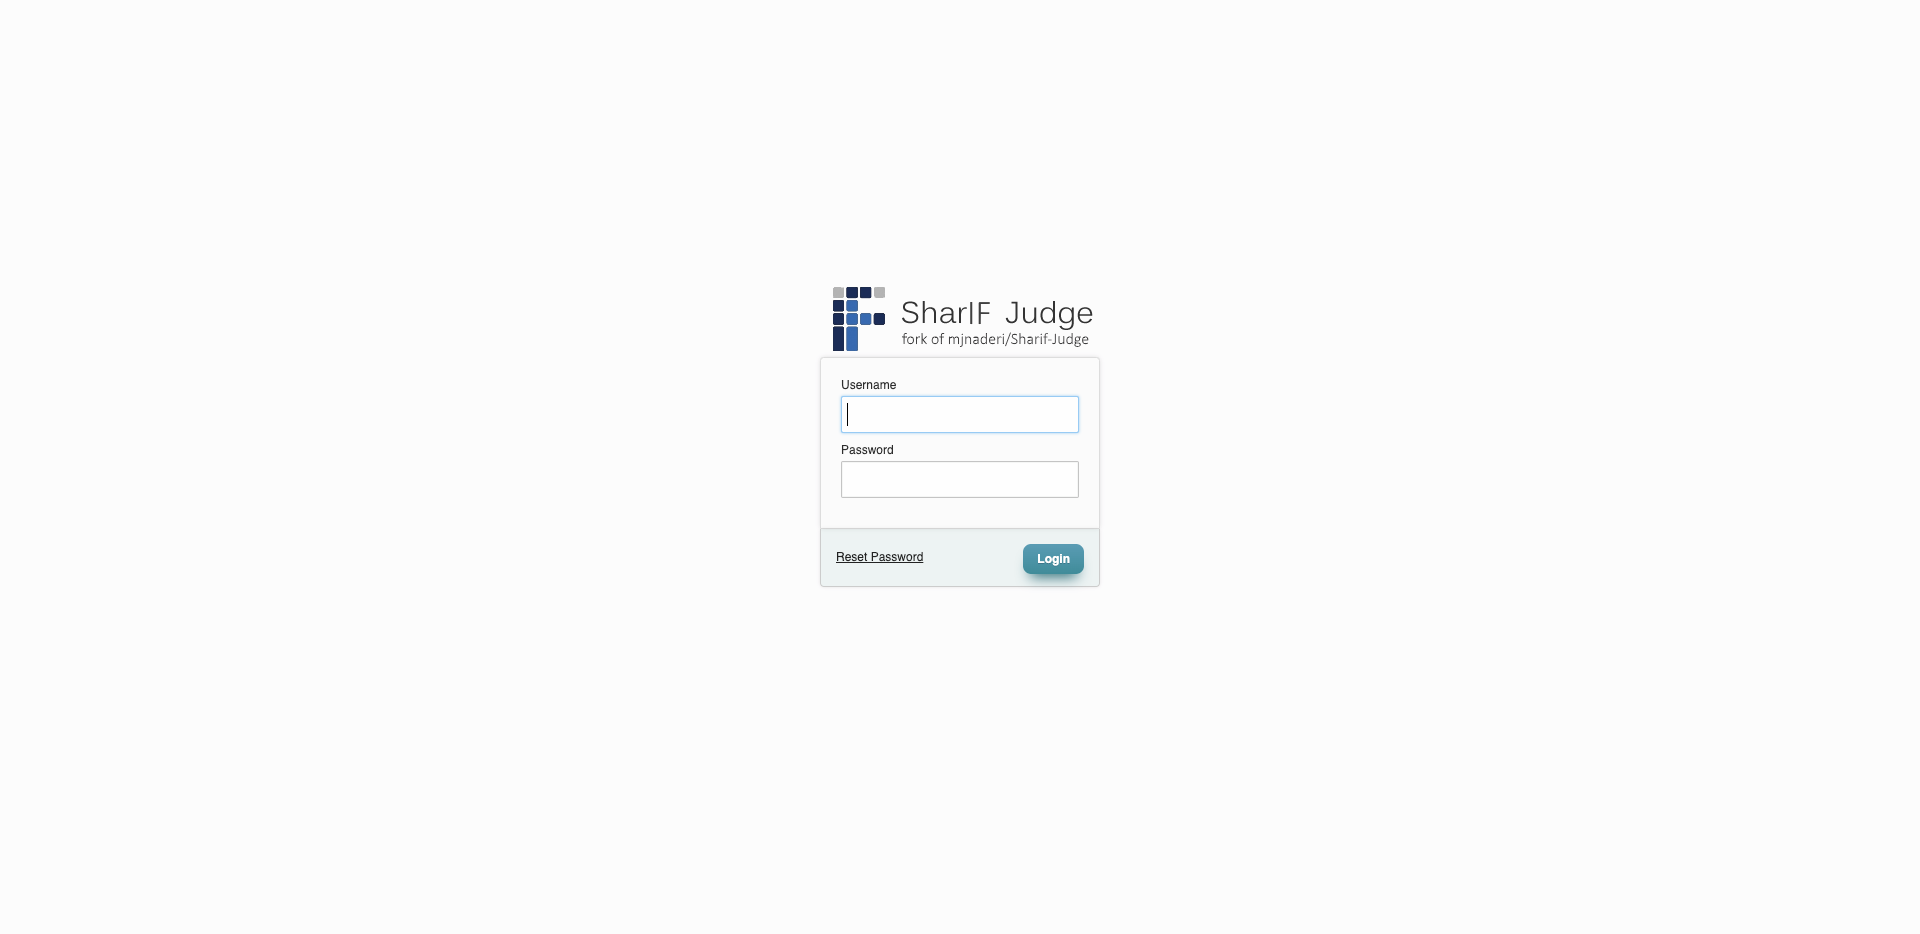
\includegraphics[scale=0.2]{login5}  
	\caption[Tampilan halaman \textit{login SharIF Judge}]{Tampilan login \textit{dashboard SharIF Judge}} 
	\label{fig:login5} 
\end{figure} 

Gambar \ref{fig:dashboard5} menunjukan hasil pengujian fungsional Halaman \textit{dashboard}
\begin{figure}[H]
	\centering  
	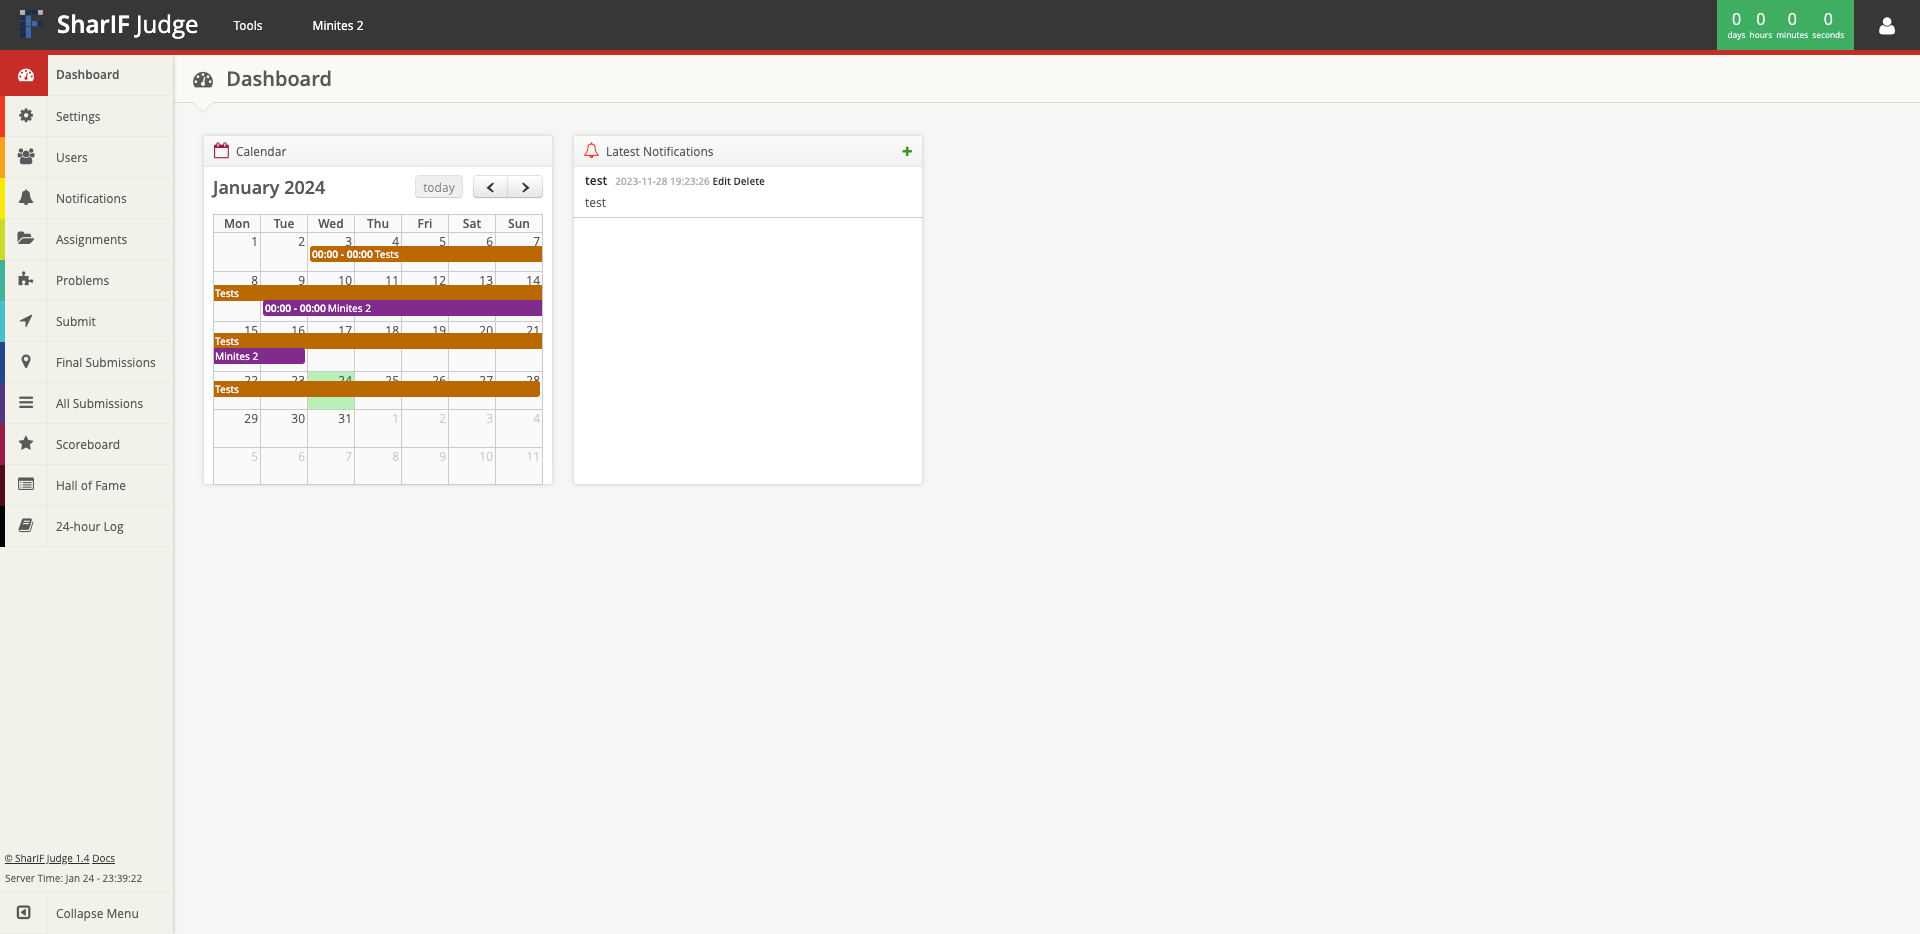
\includegraphics[scale=0.2]{dashboard5}  
	\caption[Tampilan halaman \textit{dashboard SharIF Judge}]{Tampilan \textit{dashboard SharIF Judge}} 
	\label{fig:dashboard5} 
\end{figure} 

Gambar \ref{fig:assignments5} menunjukan hasil pengujian fungsional Halaman \textit{assignments}
\begin{figure}[H]
	\centering  
	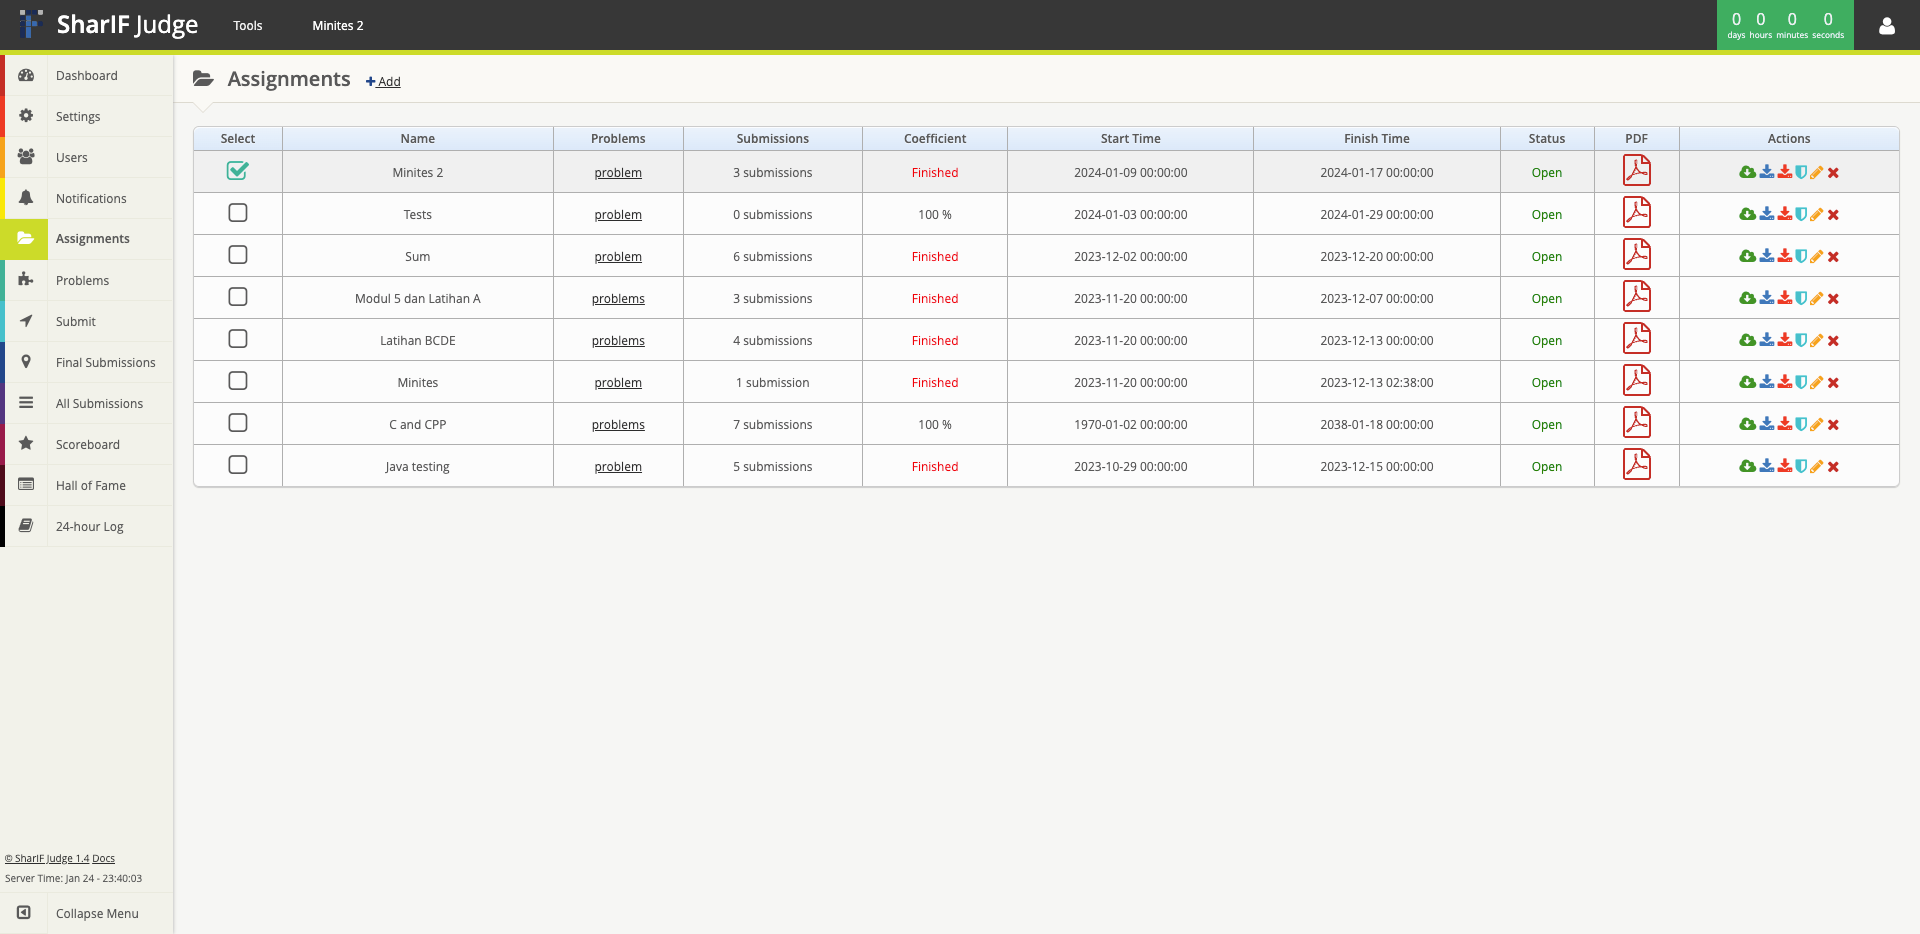
\includegraphics[scale=0.2]{assignments5}  
	\caption[Tampilan halaman \textit{assignments SharIF Judge}]{Tampilan  \textit{assignments SharIF Judge}} 
	\label{fig:assignments5} 
\end{figure} 

Gambar \ref{fig:addassignments5} menunjukan hasil pengujian fungsional Halaman \textit{add assignments}
\begin{figure}[H]
	\centering  
	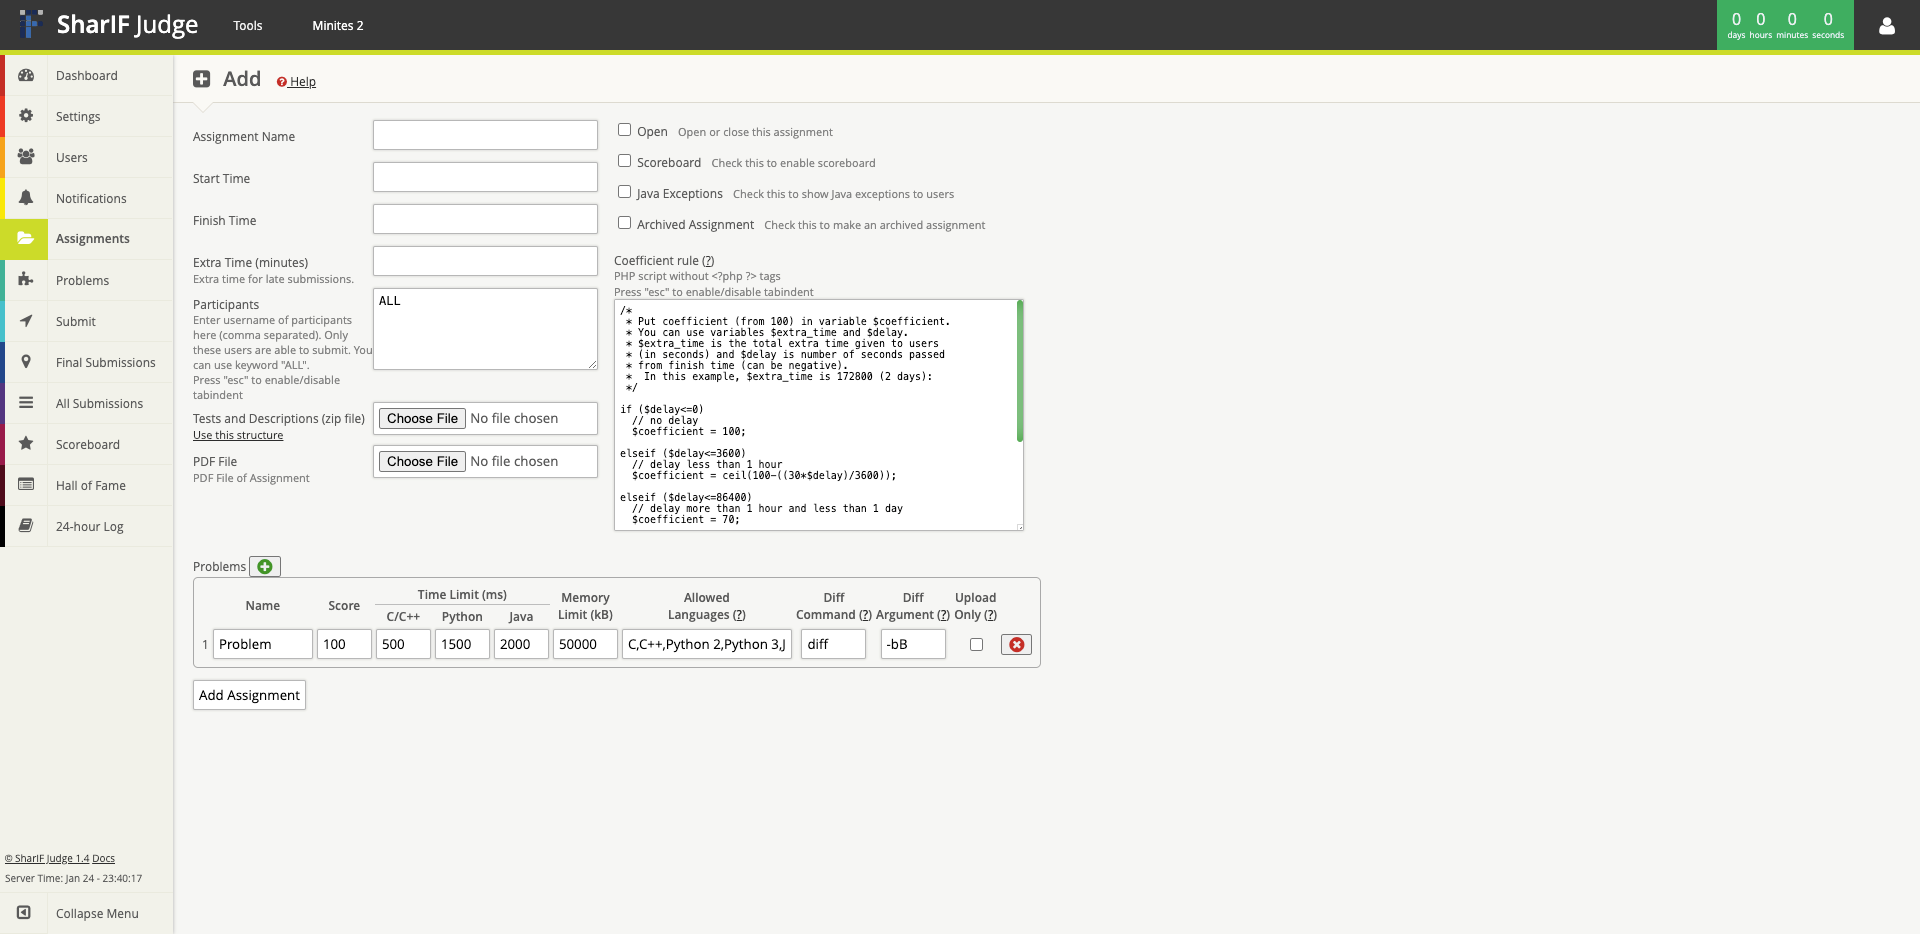
\includegraphics[scale=0.2]{addassignments5}  
	\caption[Tampilan halaman \textit{add assignments SharIF Judge}]{Tampilan  \textit{add assignments SharIF Judge}} 
	\label{fig:addassignments5} 
\end{figure} 

Gambar \ref{fig:allsub5} menunjukan hasil pengujian fungsional Halaman \textit{all submissions}
\begin{figure}[H]
	\centering  
	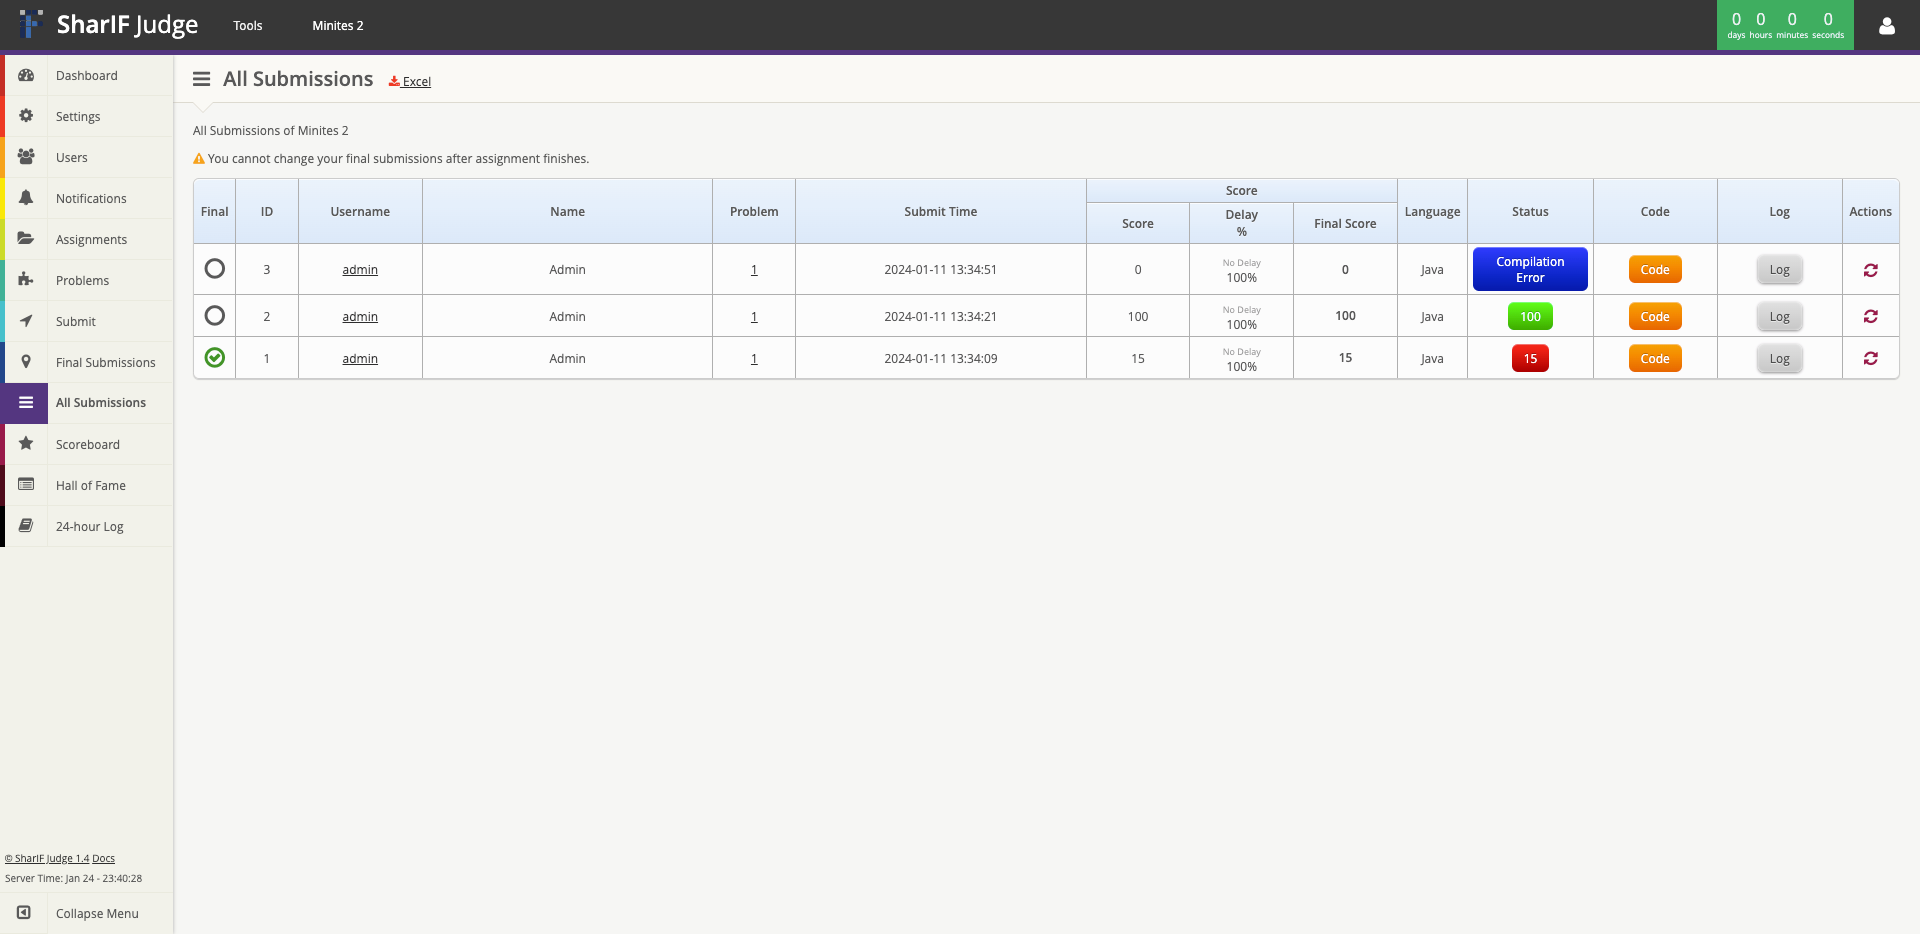
\includegraphics[scale=0.2]{allsub5}  
	\caption[Tampilan halaman \textit{all submissions SharIF Judge}]{Tampilan  \textit{all submissions SharIF Judge}} 
	\label{fig:allsub5} 
\end{figure} 

\section{Pengujian Eksperimental}
Pengujian dimulai dengan melakukan wawancara kepada admin Lab FTIS untuk menanyakan sistem operasi yang digunakan untuk menjalankan \textit{SharIF Judge}. Wawancara tersebut menghasilkan jawaban dimana \textit{SharIF Judge} dijalankan pada sistem operasi \textit{Ubuntu} versi 16.04. Versi \textit{Ubuntu} tersebut sudah tidak mendapat dukungan sehingga tidak digunakan untuk pembangunan perangkat lunak. Pengujian dilakukan untuk mengetahui apakah \textit{SharIF Judge} dapat dijalankan pada beberapa versi \textit{Ubuntu} yang berbeda. 

Pengujian pertama kali dilakukan pada sistem operasi \textit{Ubuntu} versi 22.04. Pengujian dilakukan dengan melakukan instalasi perangkat lunak \textit{SharIF Judge} dan melakukan pengamanan terhadap \textit{sandbox}. Setelah dilakukakan instalasi terdapat persoalan dalam membangun \textit{sandbox} dimana \textit{sandbox} tidak dapat dibangun dan mengembalikan \textit{error}. Oleh karena itu, dilakukan sebuah wawancara kepada admin Lab FTIS untuk menanyakan sistem operasi yang digunakan untuk menjalankan \textit{SharIF Judge}. Wawancara tersebut menghasilkan jawaban bahwa sistem operasi yang digunakan untuk menjalankan \textit{SharIF Judge} adalah \textit{Ubuntu} versi 16.04.

Pengujian selanjutnya dilakukan dengan melakukan \textit{downgrade} sistem operasi menuju \textit{Ubuntu} versi 20.04. Perangkat lunak dapat berjalan dengan baik tanpa masalah pada \textit{Ubuntu} versi 20.04. Pengujian kemudian dilanjutkan dengan melakukan pengujian eksperimental untuk menguji setiap versi sistem operasi \textit{Ubuntu} terbaru. Pengujian eksperimental dilakukan pada tiga buah versi sistem operasi \textit{Ubuntu} yakni versi 22.04, 23.04, dan 22.10. Pengujian ini bertujuan untuk menguji perangkat lunak apakah dapat berjalan pada sistem operasi yang berbeda.

\subsection{\textit{Ubuntu} 22.04}
Pengujian eksperimental pertama dilakukan pada sistem operasi \textit{Ubuntu} dengan versi 22.04. Pengujian dilakukan dengan melakukan instalasi dan melakukan pengamanan terhadap \textit{sandbox}. Setelah dilakukan instalasi terdapat persoalan dalam melakukan pengamanan terhadap \textit{sandbox}. Berikut merupakan persoalan yang didapatkan:
\subsubsection{\textit{Sandbox} tidak terbangun}
Pengujian dilakukan dengan membangun \textit{sandbox} untuk kode C/C++. Pembangunan \textit{sandbox} dilakukan pada direktori \texttt{tester/easysandbox} dengan menjalankan kode berikut:
\begin{lstlisting}[caption=Pembangunan \textit{sandbox} pada \textit{Ubuntu} 22.04, label=kode:sandbox2204]
$ cd tester/easysandbox
$ chmod +x runalltests.sh
$ chmod +x runtest.sh
$ make runtests
\end{lstlisting}

Kode \ref{kode:sandbox2204} memindahkan pengguna menuju direktori \texttt{tester/easysandbox}. Selanjutnya akses \textit{file} \texttt{runalltests} dan \texttt{runtest} diubah agar dapat dieksekusi. Terakhir \textit{file} \texttt{runtests} dijalankan menggunakan sintaks \texttt{make}. Pembangunan \textit{sandbox} menghasilkan pesan berupa \texttt{All tests passed!}. Namun pada sistem operasi ini, \textit{sandbox} tidak dapat dibentuk dan menghasilkan \textit{error message} seperti yang ditunjukan pada Kode \ref{kode:errormsg2204}.
\begin{lstlisting}[caption=\textit{Error message} pembangunan \textit{sandbox} pada \textit{Ubuntu} 22.04, label=kode:errormsg2204]
./runalltests.sh t/test01 t/test02 t/test03 t/test04 t/test05 t/test06 t/test07 t/test08 t/test09 t/test10 t/test11 t/test12 t/test13 t/test14
Executing t/test01...passed!
Executing t/test02...passed!
Executing t/test03...passed!
Executing t/test04...passed!
Executing t/test05...passed!
Executing t/test06...passed!
Executing t/test07...passed!
Executing t/test08...passed!
Executing t/test09...1a2
> Hello, C++ world
failed (output mismatch, expected [<<entering SECCOMP mode>>
Hello, C++ world], got [<<entering SECCOMP mode>>])
Executing t/test10...1a2
> Hello from the constructor!
failed (output mismatch, expected [<<entering SECCOMP mode>>
Hello from the constructor!], got [<<entering SECCOMP mode>>])
Executing t/test11...passed!
Executing t/test12...1a2,3
> Here we are in main()
> Hello from the destructor!
failed (output mismatch, expected [<<entering SECCOMP mode>>
Here we are in main()
Hello from the destructor!], got [<<entering SECCOMP mode>>])
Executing t/test13...passed!
Executing t/test14...1a2
> 500500
failed (output mismatch, expected [<<entering SECCOMP mode>>
500500], got [<<entering SECCOMP mode>>])
4 test(s) failed
make: *** [Makefile:31: runtests] Error 1
\end{lstlisting}
Kode \ref{kode:errormsg2204} merupakan keluaran dari pembangunan \textit{sandbox} pada \textit{Ubuntu} 22.04. Terdapat \textit{error message} berupa keluaran tidak sesuai dengan yang seharusnya. Pembangunan dapat dikatakan tidak berhasil karena hanya sebagian \textit{test case} yang berhasil dilewati dan tidak terdapat pesan berupa \texttt{All tests passed!}. \textit{Error message} ini dihasilkan karena terdapat perbedaan versi pada \textit{seccomp} atau \textit{secure computing mode} sehingga tidak dapat dijalankan pada versi teratas pada \textit{Ubuntu}.

\subsection{\textit{Ubuntu} 23.04}
Pengujian eksperimental kedua dilakukan pada sistem operasi \textit{Ubuntu} dengan versi 23.04. Pengujian dilakukan dengan melakukan instalasi dan melakukan pengamanan terhadap \textit{sandbox}. Setelah dilakukan instalasi terdapat persoalan dalam melakukan pengamanan terhadap \textit{sandbox}. Berikut merupakan persoalan yang didapatkan:
\begin{lstlisting}[caption=Pembangunan \textit{sandbox} pada \textit{Ubuntu} 23.04, label=kode:sandbox2304]
$ cd tester/easysandbox
$ chmod +x runalltests.sh
$ chmod +x runtest.sh
$ make runtests
\end{lstlisting}

Kode \ref{kode:sandbox2304} memindahkan pengguna menuju direktori \texttt{tester/easysandbox}. Selanjutnya akses \textit{file} \texttt{runalltests} dan \texttt{runtest} diubah agar dapat dieksekusi. Terakhir \textit{file} \texttt{runtests} dijalankan menggunakan sintaks \texttt{make}. Pembangunan \textit{sandbox} menghasilkan pesan berupa \texttt{All tests passed!}. Namun pada sistem operasi ini, \textit{sandbox} tidak dapat dibentuk dan menghasilkan \textit{error message} seperti yang ditunjukan pada Kode \ref{kode:errormsg2304}.
\begin{lstlisting}[caption=\textit{Error message} pembangunan \textit{sandbox} pada \textit{Ubuntu} 23.04, label=kode:errormsg2304]
/runalltests.sh t/test01 t/test02 t/test03 t/test04 t/test05 t/test06 t/test07 t/test08 t/test09 t/test10 t/test11 t/test12 t/test13 t/test14
Executing t/test01...failed (exit code mismatch, expected 0, got 139)
Executing t/test02...1a2
> Hello, world
failed (output mismatch, expected [<<entering SECCOMP mode>>
Hello, world], got [<<entering SECCOMP mode>>])
Executing t/test03...failed (exit code mismatch, expected 137, got 139)
Executing t/test04...1a2
> 500500
failed (output mismatch, expected [<<entering SECCOMP mode>>
500500], got [<<entering SECCOMP mode>>])
Executing t/test05...1a2
> Hello, world
failed (output mismatch, expected [<<entering SECCOMP mode>>
Hello, world], got [<<entering SECCOMP mode>>])
Executing t/test06...failed (exit code mismatch, expected 137, got 139)
Executing t/test07...1a2
> 59
failed (output mismatch, expected [<<entering SECCOMP mode>>
59], got [<<entering SECCOMP mode>>])
Executing t/test08...failed (exit code mismatch, expected 0, got 139)
Executing t/test09...1a2
> Hello, C++ world
failed (output mismatch, expected [<<entering SECCOMP mode>>
Hello, C++ world], got [<<entering SECCOMP mode>>])
Executing t/test10...1a2
> Hello from the constructor!
failed (output mismatch, expected [<<entering SECCOMP mode>>
Hello from the constructor!], got [<<entering SECCOMP mode>>])
Executing t/test11...failed (exit code mismatch, expected 137, got 139)
Executing t/test12...1a2,3
> Here we are in main()
> Hello from the destructor!
failed (output mismatch, expected [<<entering SECCOMP mode>>
Here we are in main()
Hello from the destructor!], got [<<entering SECCOMP mode>>])
Executing t/test13...1a2
> Hello from the destructor!
failed (output mismatch, expected [<<entering SECCOMP mode>>
Hello from the destructor!], got [<<entering SECCOMP mode>>])
Executing t/test14...1a2
> 500500
failed (output mismatch, expected [<<entering SECCOMP mode>>
500500], got [<<entering SECCOMP mode>>])
14 test(s) failed
make: *** [Makefile:31: runtests] Error 1
\end{lstlisting}
Kode \ref{kode:errormsg2304} merupakan keluaran dari pembangunan \textit{sandbox} pada \textit{Ubuntu} 23.04. Terdapat \textit{error message} berupa keluaran tidak sesuai dengan yang seharusnya. Pembangunan dapat dikatakan tidak berhasil karena seluruh \textit{test case} tidak berhasil dilewati dan tidak terdapat pesan berupa \texttt{All tests passed!}. \textit{Error message} ini dihasilkan karena terdapat perbedaan versi pada \textit{seccomp} atau \textit{secure computing mode} sehingga tidak dapat dijalankan pada versi teratas pada \textit{Ubuntu}.

\subsection{\textit{Ubuntu} 23.10}
Pengujian eksperimental ketiga dilakukan pada sistem operasi \textit{Ubuntu} dengan versi 23.10. Pengujian dilakukan dengan melakukan instalasi dan melakukan pengamanan terhadap \textit{sandbox}. Setelah dilakukan instalasi terdapat persoalan dalam melakukan pengamanan terhadap \textit{sandbox}. Berikut merupakan persoalan yang didapatkan:
\begin{lstlisting}[caption=Pembangunan \textit{sandbox} pada \textit{Ubuntu} 23.10, label=kode:sandbox2310]
$ cd tester/easysandbox
$ chmod +x runalltests.sh
$ chmod +x runtest.sh
$ make runtests
\end{lstlisting}

Kode \ref{kode:sandbox2310} memindahkan pengguna menuju direktori \texttt{tester/easysandbox}. Selanjutnya akses \textit{file} \texttt{runalltests} dan \texttt{runtest} diubah agar dapat dieksekusi. Terakhir \textit{file} \texttt{runtests} dijalankan menggunakan sintaks \texttt{make}. Pembangunan \textit{sandbox} menghasilkan pesan berupa \texttt{All tests passed!}. Namun pada sistem operasi ini, \textit{sandbox} tidak dapat dibentuk dan menghasilkan \textit{error message} seperti yang dijunukan pada Kode \ref{kode:errormsg2310}.
\begin{lstlisting}[caption=\textit{Error message} pembangunan \textit{sandbox} pada \textit{Ubuntu} 23.10, label=kode:errormsg2310]
g++ -g -Wall -D_BSD_SOURCE  -o t/test09 t/test09.cpp
In file included from /usr/include/x86_64-linux-gnu/c++/13/bits/os_defines.h:39,
                 from /usr/include/x86_64-linux-gnu/c++/13/bits/c++config.h:679,
                 from /usr/include/c++/13/bits/requires_hosted.h:31,
                 from /usr/include/c++/13/iostream:38,
                 from t/test09.cpp:3:
/usr/include/features.h:196:3: warning: #warning "_BSD_SOURCE and _SVID_SOURCE are deprecated, use _DEFAULT_SOURCE" [-Wcpp]
  196 | # warning "_BSD_SOURCE and _SVID_SOURCE are deprecated, use _DEFAULT_SOURCE"
      |   ^~~~~~~
g++ -g -Wall -D_BSD_SOURCE  -o t/test10 t/test10.cpp
In file included from /usr/include/x86_64-linux-gnu/c++/13/bits/os_defines.h:39,
                 from /usr/include/x86_64-linux-gnu/c++/13/bits/c++config.h:679,
                 from /usr/include/c++/13/bits/requires_hosted.h:31,
                 from /usr/include/c++/13/iostream:38,
                 from t/test10.cpp:3:
/usr/include/features.h:196:3: warning: #warning "_BSD_SOURCE and _SVID_SOURCE are deprecated, use _DEFAULT_SOURCE" [-Wcpp]
  196 | # warning "_BSD_SOURCE and _SVID_SOURCE are deprecated, use _DEFAULT_SOURCE"
      |   ^~~~~~~
g++ -g -Wall -D_BSD_SOURCE  -o t/test11 t/test11.cpp
In file included from /usr/include/x86_64-linux-gnu/c++/13/bits/os_defines.h:39,
                 from /usr/include/x86_64-linux-gnu/c++/13/bits/c++config.h:679,
                 from /usr/include/c++/13/bits/requires_hosted.h:31,
                 from /usr/include/c++/13/iostream:38,
                 from t/test11.cpp:4:
/usr/include/features.h:196:3: warning: #warning "_BSD_SOURCE and _SVID_SOURCE are deprecated, use _DEFAULT_SOURCE" [-Wcpp]
  196 | # warning "_BSD_SOURCE and _SVID_SOURCE are deprecated, use _DEFAULT_SOURCE"
      |   ^~~~~~~
g++ -g -Wall -D_BSD_SOURCE  -o t/test12 t/test12.cpp
In file included from /usr/include/x86_64-linux-gnu/c++/13/bits/os_defines.h:39,
                 from /usr/include/x86_64-linux-gnu/c++/13/bits/c++config.h:679,
                 from /usr/include/c++/13/bits/requires_hosted.h:31,
                 from /usr/include/c++/13/iostream:38,
                 from t/test12.cpp:3:
/usr/include/features.h:196:3: warning: #warning "_BSD_SOURCE and _SVID_SOURCE are deprecated, use _DEFAULT_SOURCE" [-Wcpp]
  196 | # warning "_BSD_SOURCE and _SVID_SOURCE are deprecated, use _DEFAULT_SOURCE"
      |   ^~~~~~~
gcc -std=c99 -g -Wall -D_BSD_SOURCE   -o t/test13 t/test13.c
In file included from /usr/include/x86_64-linux-gnu/bits/libc-header-start.h:33,
                 from /usr/include/stdio.h:27,
                 from t/test13.c:3:
/usr/include/features.h:196:3: warning: #warning "_BSD_SOURCE and _SVID_SOURCE are deprecated, use _DEFAULT_SOURCE" [-Wcpp]
  196 | # warning "_BSD_SOURCE and _SVID_SOURCE are deprecated, use _DEFAULT_SOURCE"
      |   ^~~~~~~
g++ -g -Wall -D_BSD_SOURCE  -o t/test14 t/test14.cpp
In file included from /usr/include/x86_64-linux-gnu/c++/13/bits/os_defines.h:39,
                 from /usr/include/x86_64-linux-gnu/c++/13/bits/c++config.h:679,
                 from /usr/include/c++/13/bits/requires_hosted.h:31,
                 from /usr/include/c++/13/iostream:38,
                 from t/test14.cpp:4:
/usr/include/features.h:196:3: warning: #warning "_BSD_SOURCE and _SVID_SOURCE are deprecated, use _DEFAULT_SOURCE" [-Wcpp]
  196 | # warning "_BSD_SOURCE and _SVID_SOURCE are deprecated, use _DEFAULT_SOURCE"
      |   ^~~~~~~
./runalltests.sh t/test01 t/test02 t/test03 t/test04 t/test05 t/test06 t/test07 t/test08 t/test09 t/test10 t/test11 t/test12 t/test13 t/test14
Executing t/test01...failed (exit code mismatch, expected 0, got 139)
Executing t/test02...1a2
> Hello, world
failed (output mismatch, expected [<<entering SECCOMP mode>>
Hello, world], got [<<entering SECCOMP mode>>])
Executing t/test03...failed (exit code mismatch, expected 137, got 139)
Executing t/test04...1a2
> 500500
failed (output mismatch, expected [<<entering SECCOMP mode>>
500500], got [<<entering SECCOMP mode>>])
Executing t/test05...1a2
> Hello, world
failed (output mismatch, expected [<<entering SECCOMP mode>>
Hello, world], got [<<entering SECCOMP mode>>])
Executing t/test06...failed (exit code mismatch, expected 137, got 139)
Executing t/test07...1a2
> 59
failed (output mismatch, expected [<<entering SECCOMP mode>>
59], got [<<entering SECCOMP mode>>])
Executing t/test08...failed (exit code mismatch, expected 0, got 139)
Executing t/test09...1a2
> Hello, C++ world
failed (output mismatch, expected [<<entering SECCOMP mode>>
Hello, C++ world], got [<<entering SECCOMP mode>>])
Executing t/test10...1a2
> Hello from the constructor!
failed (output mismatch, expected [<<entering SECCOMP mode>>
Hello from the constructor!], got [<<entering SECCOMP mode>>])
Executing t/test11...failed (exit code mismatch, expected 137, got 139)
Executing t/test12...1a2,3
> Here we are in main()
> Hello from the destructor!
failed (output mismatch, expected [<<entering SECCOMP mode>>
Here we are in main()
Hello from the destructor!], got [<<entering SECCOMP mode>>])
Executing t/test13...1a2
> Hello from the destructor!
failed (output mismatch, expected [<<entering SECCOMP mode>>
Hello from the destructor!], got [<<entering SECCOMP mode>>])
Executing t/test14...1a2
> 500500
failed (output mismatch, expected [<<entering SECCOMP mode>>
500500], got [<<entering SECCOMP mode>>])
14 test(s) failed
make: *** [Makefile:31: runtests] Error 1
\end{lstlisting}
Kode \ref{kode:errormsg2310} merupakan keluaran dari pembangunan \textit{sandbox} pada \textit{Ubuntu} 23.10. Terdapat \textit{error message} berupa \textit{warning} dan \textit{test case} yang tidak berhasil dijalankan. Pembangunan dapat dikatakan tidak berhasil karena seluruh \textit{test case} tidak berhasil dilewati dan tidak terdapat pesan berupa \texttt{All tests passed!}. \textit{Error message} ini dihasilkan karena terdapat perbedaan versi pada \textit{seccomp} atau \textit{secure computing mode} sehingga tidak dapat dijalankan pada versi teratas pada \textit{Ubuntu}.
